\documentclass[11pt,a4paper]{article}
% Most compatible output (PDF 1.4, no object or xref streams) for browser and GitHub viewers
\pdfminorversion=4
\pdfobjcompresslevel=0

\usepackage[T1]{fontenc}
\usepackage[utf8]{inputenc}
\usepackage{lmodern}
\usepackage{microtype}
\usepackage[margin=2.5cm]{geometry}
\usepackage{amsmath,amssymb}
\usepackage{booktabs}
\usepackage{tabularx}
\usepackage{siunitx}
\usepackage{graphicx}
\usepackage{xcolor}
\usepackage{pgfplots}
\pgfplotsset{compat=1.17}
\usetikzlibrary{positioning}
\usepackage[ruled,vlined,linesnumbered]{algorithm2e}
\usepackage{listings}
\usepackage{xspace}
\usepackage[colorlinks=true,linkcolor=blue!50!black,citecolor=green!40!black,urlcolor=blue!60!black]{hyperref}
\usepackage[nameinlink]{cleveref}
\hypersetup{
  pdftitle={From a 2010 Prototype to Contraction Hierarchies in Three Languages},
  pdfauthor={Nick Dinges},
  pdfsubject={Engineering k shortest paths with Eppstein, Yen-Lawler, arc flags and PHAST in C\#, Go and Rust; an experiment with Claude},
  pdfkeywords={k shortest paths, Eppstein, Yen, contraction hierarchies, PHAST, arc flags, garbage collection, Rust, Go, C\#, AI-assisted development}
}

\sisetup{group-separator={,},group-minimum-digits=4}
\lstset{basicstyle=\ttfamily\small,columns=fullflexible,breaklines=true,frame=single,framerule=0.3pt}
\newcommand{\cs}{C\#}
\newcommand{\eg}{e.\,g.\@\xspace}
\newcommand{\ie}{i.\,e.\@\xspace}
% \val{scenario/language/field}: a measured value from paper/data/*.csv (see scripts/make_tables.py)
\newcommand{\val}[1]{\ifcsname val@#1\endcsname\csname val@#1\endcsname\else\errmessage{Unknown value: #1}\fi}

\newcommand{\NumArcFlagsGainFour}{15--21}
\newcommand{\NumArcFlagsGainSixteen}{15--25}
\newcommand{\NumChBreakEven}{310--520}
\newcommand{\NumCorridorSpeedup}{31--148}
\newcommand{\NumCpu}{Intel Xeon Processor @ 2.10GHz}
\newcommand{\NumCsSecondOverSteadyMax}{5.0}
\newcommand{\NumDays}{8--10 November 2026}
\newcommand{\NumDotnet}{10.0.114}
\newcommand{\NumGcShareCs}{4}
\newcommand{\NumGcShareCsYen}{4}
\newcommand{\NumGo}{Go~1.24.7}
\newcommand{\NumLocCs}{1825}
\newcommand{\NumLocCsTests}{1212}
\newcommand{\NumLocGo}{1851}
\newcommand{\NumLocGoTests}{1733}
\newcommand{\NumLocRust}{1988}
\newcommand{\NumLocRustTests}{352}
\newcommand{\NumLocalRatioRepeated}{0.52\,ms}
\newcommand{\NumLocalRepeated}{75\,ms}
\newcommand{\NumMaxRatioNext}{5.1}
\newcommand{\NumMaxRatioSecond}{5.2}
\newcommand{\NumMaxRatioTreeAll}{4.4}
\newcommand{\NumMaxRatioTreeAllScenario}{local-1000-ratio}
\newcommand{\NumMaxRatioTreeBig}{1.2}
\newcommand{\NumMaxRatioTreeLong}{1.6}
\newcommand{\NumOutputShare}{95--99}
\newcommand{\NumPerPathMicros}{28--32}
\newcommand{\NumPerWeightMicros}{0.3--1.4}
\newcommand{\NumPhastSpeedupBig}{2.4--3.6}
\newcommand{\NumPhastSpeedupSmall}{2.1--4.0}
\newcommand{\NumPullRequests}{11}
\newcommand{\NumRatioTreeShort}{4.4}
\newcommand{\NumRepeat}{5}
\newcommand{\NumRssRatio}{1.6--1.8}
\newcommand{\NumRustEnumAdvantage}{9--12}
\newcommand{\NumRustc}{1.97.0}
\newcommand{\NumSessions}{three}
\newcommand{\NumSpreadMax}{81}
\newcommand{\NumSpreadMedian}{15}
\newcommand{\NumSpreadNinety}{30}
\newcommand{\NumVOneFirst}{40.3\,s}
\newcommand{\NumVOneSize}{12}
\newcommand{\NumVTwoFirst}{0.12\,ms}
\expandafter\def\csname val@arcflags-16-200-two-way/cs/alloc\endcsname{0.00}
\expandafter\def\csname val@arcflags-16-200-two-way/cs/arcflags\endcsname{45{,}264}
\expandafter\def\csname val@arcflags-16-200-two-way/cs/arcflags:s\endcsname{45}
\expandafter\def\csname val@arcflags-16-200-two-way/cs/build\endcsname{31}
\expandafter\def\csname val@arcflags-16-200-two-way/cs/first\endcsname{17.9}
\expandafter\def\csname val@arcflags-16-200-two-way/cs/gc\endcsname{0}
\expandafter\def\csname val@arcflags-16-200-two-way/cs/mem\endcsname{10.0}
\expandafter\def\csname val@arcflags-16-200-two-way/cs/next\endcsname{0.00}
\expandafter\def\csname val@arcflags-16-200-two-way/cs/pause\endcsname{0.00}
\expandafter\def\csname val@arcflags-16-200-two-way/cs/rss\endcsname{61}
\expandafter\def\csname val@arcflags-16-200-two-way/cs/second\endcsname{7.3}
\expandafter\def\csname val@arcflags-16-200-two-way/cs/warm\endcsname{6.7}
\expandafter\def\csname val@arcflags-16-200-two-way/cs/warmlo\endcsname{6.7}
\expandafter\def\csname val@arcflags-16-200-two-way/go/alloc\endcsname{0.00}
\expandafter\def\csname val@arcflags-16-200-two-way/go/arcflags\endcsname{52{,}658}
\expandafter\def\csname val@arcflags-16-200-two-way/go/arcflags:s\endcsname{53}
\expandafter\def\csname val@arcflags-16-200-two-way/go/build\endcsname{57}
\expandafter\def\csname val@arcflags-16-200-two-way/go/first\endcsname{8.2}
\expandafter\def\csname val@arcflags-16-200-two-way/go/gc\endcsname{0}
\expandafter\def\csname val@arcflags-16-200-two-way/go/mem\endcsname{5.9}
\expandafter\def\csname val@arcflags-16-200-two-way/go/next\endcsname{0.00}
\expandafter\def\csname val@arcflags-16-200-two-way/go/pause\endcsname{0.00}
\expandafter\def\csname val@arcflags-16-200-two-way/go/rss\endcsname{24.8}
\expandafter\def\csname val@arcflags-16-200-two-way/go/second\endcsname{9.4}
\expandafter\def\csname val@arcflags-16-200-two-way/go/warm\endcsname{7.9}
\expandafter\def\csname val@arcflags-16-200-two-way/go/warmlo\endcsname{7.9}
\expandafter\def\csname val@arcflags-16-200-two-way/range/alloc\endcsname{0.00--0.00}
\expandafter\def\csname val@arcflags-16-200-two-way/range/arcflags\endcsname{45{,}263--52{,}658}
\expandafter\def\csname val@arcflags-16-200-two-way/range/arcflags:s\endcsname{45--53}
\expandafter\def\csname val@arcflags-16-200-two-way/range/build\endcsname{13.8--57}
\expandafter\def\csname val@arcflags-16-200-two-way/range/first\endcsname{7.4--17.9}
\expandafter\def\csname val@arcflags-16-200-two-way/range/gc\endcsname{0.00--0.00}
\expandafter\def\csname val@arcflags-16-200-two-way/range/mem\endcsname{5.9--11.9}
\expandafter\def\csname val@arcflags-16-200-two-way/range/next\endcsname{0.00--0.00}
\expandafter\def\csname val@arcflags-16-200-two-way/range/pause\endcsname{0.00--0.00}
\expandafter\def\csname val@arcflags-16-200-two-way/range/rss\endcsname{18.3--61}
\expandafter\def\csname val@arcflags-16-200-two-way/range/second\endcsname{6.8--9.4}
\expandafter\def\csname val@arcflags-16-200-two-way/range/warm\endcsname{6.7--7.9}
\expandafter\def\csname val@arcflags-16-200-two-way/rust/alloc\endcsname{0.00}
\expandafter\def\csname val@arcflags-16-200-two-way/rust/arcflags\endcsname{45{,}263}
\expandafter\def\csname val@arcflags-16-200-two-way/rust/arcflags:s\endcsname{45}
\expandafter\def\csname val@arcflags-16-200-two-way/rust/build\endcsname{13.8}
\expandafter\def\csname val@arcflags-16-200-two-way/rust/first\endcsname{7.4}
\expandafter\def\csname val@arcflags-16-200-two-way/rust/gc\endcsname{0}
\expandafter\def\csname val@arcflags-16-200-two-way/rust/mem\endcsname{11.9}
\expandafter\def\csname val@arcflags-16-200-two-way/rust/next\endcsname{0.00}
\expandafter\def\csname val@arcflags-16-200-two-way/rust/pause\endcsname{0.00}
\expandafter\def\csname val@arcflags-16-200-two-way/rust/rss\endcsname{18.3}
\expandafter\def\csname val@arcflags-16-200-two-way/rust/second\endcsname{6.8}
\expandafter\def\csname val@arcflags-16-200-two-way/rust/warm\endcsname{6.9}
\expandafter\def\csname val@arcflags-16-200-two-way/rust/warmlo\endcsname{6.9}
\expandafter\def\csname val@arcflags-4-200-two-way/cs/alloc\endcsname{0.00}
\expandafter\def\csname val@arcflags-4-200-two-way/cs/arcflags\endcsname{11{,}199}
\expandafter\def\csname val@arcflags-4-200-two-way/cs/arcflags:s\endcsname{11.2}
\expandafter\def\csname val@arcflags-4-200-two-way/cs/build\endcsname{30}
\expandafter\def\csname val@arcflags-4-200-two-way/cs/first\endcsname{16.9}
\expandafter\def\csname val@arcflags-4-200-two-way/cs/gc\endcsname{0}
\expandafter\def\csname val@arcflags-4-200-two-way/cs/mem\endcsname{8.0}
\expandafter\def\csname val@arcflags-4-200-two-way/cs/next\endcsname{0.00}
\expandafter\def\csname val@arcflags-4-200-two-way/cs/pause\endcsname{0.00}
\expandafter\def\csname val@arcflags-4-200-two-way/cs/rss\endcsname{61}
\expandafter\def\csname val@arcflags-4-200-two-way/cs/second\endcsname{7.5}
\expandafter\def\csname val@arcflags-4-200-two-way/cs/warm\endcsname{6.8}
\expandafter\def\csname val@arcflags-4-200-two-way/cs/warmlo\endcsname{5.7}
\expandafter\def\csname val@arcflags-4-200-two-way/go/alloc\endcsname{0.00}
\expandafter\def\csname val@arcflags-4-200-two-way/go/arcflags\endcsname{12{,}617}
\expandafter\def\csname val@arcflags-4-200-two-way/go/arcflags:s\endcsname{12.6}
\expandafter\def\csname val@arcflags-4-200-two-way/go/build\endcsname{25.9}
\expandafter\def\csname val@arcflags-4-200-two-way/go/first\endcsname{9.2}
\expandafter\def\csname val@arcflags-4-200-two-way/go/gc\endcsname{0}
\expandafter\def\csname val@arcflags-4-200-two-way/go/mem\endcsname{4.0}
\expandafter\def\csname val@arcflags-4-200-two-way/go/next\endcsname{0.00}
\expandafter\def\csname val@arcflags-4-200-two-way/go/pause\endcsname{0.00}
\expandafter\def\csname val@arcflags-4-200-two-way/go/rss\endcsname{25.1}
\expandafter\def\csname val@arcflags-4-200-two-way/go/second\endcsname{10.1}
\expandafter\def\csname val@arcflags-4-200-two-way/go/warm\endcsname{8.6}
\expandafter\def\csname val@arcflags-4-200-two-way/go/warmlo\endcsname{8.1}
\expandafter\def\csname val@arcflags-4-200-two-way/range/alloc\endcsname{0.00--0.00}
\expandafter\def\csname val@arcflags-4-200-two-way/range/arcflags\endcsname{10{,}317--12{,}617}
\expandafter\def\csname val@arcflags-4-200-two-way/range/arcflags:s\endcsname{10.3--12.6}
\expandafter\def\csname val@arcflags-4-200-two-way/range/build\endcsname{13.9--30}
\expandafter\def\csname val@arcflags-4-200-two-way/range/first\endcsname{7.3--16.9}
\expandafter\def\csname val@arcflags-4-200-two-way/range/gc\endcsname{0.00--0.00}
\expandafter\def\csname val@arcflags-4-200-two-way/range/mem\endcsname{4.0--10.0}
\expandafter\def\csname val@arcflags-4-200-two-way/range/next\endcsname{0.00--0.00}
\expandafter\def\csname val@arcflags-4-200-two-way/range/pause\endcsname{0.00--0.00}
\expandafter\def\csname val@arcflags-4-200-two-way/range/rss\endcsname{16.5--61}
\expandafter\def\csname val@arcflags-4-200-two-way/range/second\endcsname{7.2--10.1}
\expandafter\def\csname val@arcflags-4-200-two-way/range/warm\endcsname{6.8--8.6}
\expandafter\def\csname val@arcflags-4-200-two-way/rust/alloc\endcsname{0.00}
\expandafter\def\csname val@arcflags-4-200-two-way/rust/arcflags\endcsname{10{,}317}
\expandafter\def\csname val@arcflags-4-200-two-way/rust/arcflags:s\endcsname{10.3}
\expandafter\def\csname val@arcflags-4-200-two-way/rust/build\endcsname{13.9}
\expandafter\def\csname val@arcflags-4-200-two-way/rust/first\endcsname{7.3}
\expandafter\def\csname val@arcflags-4-200-two-way/rust/gc\endcsname{0}
\expandafter\def\csname val@arcflags-4-200-two-way/rust/mem\endcsname{10.0}
\expandafter\def\csname val@arcflags-4-200-two-way/rust/next\endcsname{0.00}
\expandafter\def\csname val@arcflags-4-200-two-way/rust/pause\endcsname{0.00}
\expandafter\def\csname val@arcflags-4-200-two-way/rust/rss\endcsname{16.5}
\expandafter\def\csname val@arcflags-4-200-two-way/rust/second\endcsname{7.2}
\expandafter\def\csname val@arcflags-4-200-two-way/rust/warm\endcsname{7.4}
\expandafter\def\csname val@arcflags-4-200-two-way/rust/warmlo\endcsname{7.2}
\expandafter\def\csname val@build-dimacs-1000/cs/alloc\endcsname{0.00}
\expandafter\def\csname val@build-dimacs-1000/cs/arcflags\endcsname{0.00}
\expandafter\def\csname val@build-dimacs-1000/cs/build\endcsname{704}
\expandafter\def\csname val@build-dimacs-1000/cs/first\endcsname{457}
\expandafter\def\csname val@build-dimacs-1000/cs/gc\endcsname{0}
\expandafter\def\csname val@build-dimacs-1000/cs/mem\endcsname{5.3}
\expandafter\def\csname val@build-dimacs-1000/cs/next\endcsname{0.00}
\expandafter\def\csname val@build-dimacs-1000/cs/pause\endcsname{0.00}
\expandafter\def\csname val@build-dimacs-1000/cs/rss\endcsname{564}
\expandafter\def\csname val@build-dimacs-1000/cs/second\endcsname{268}
\expandafter\def\csname val@build-dimacs-1000/cs/warm\endcsname{267}
\expandafter\def\csname val@build-dimacs-1000/cs/warmlo\endcsname{258}
\expandafter\def\csname val@build-dimacs-1000/go/alloc\endcsname{0.00}
\expandafter\def\csname val@build-dimacs-1000/go/arcflags\endcsname{0.00}
\expandafter\def\csname val@build-dimacs-1000/go/build\endcsname{1{,}020}
\expandafter\def\csname val@build-dimacs-1000/go/build:s\endcsname{1.0}
\expandafter\def\csname val@build-dimacs-1000/go/first\endcsname{381}
\expandafter\def\csname val@build-dimacs-1000/go/gc\endcsname{0}
\expandafter\def\csname val@build-dimacs-1000/go/mem\endcsname{54}
\expandafter\def\csname val@build-dimacs-1000/go/next\endcsname{0.00}
\expandafter\def\csname val@build-dimacs-1000/go/pause\endcsname{0.00}
\expandafter\def\csname val@build-dimacs-1000/go/rss\endcsname{350}
\expandafter\def\csname val@build-dimacs-1000/go/second\endcsname{349}
\expandafter\def\csname val@build-dimacs-1000/go/warm\endcsname{341}
\expandafter\def\csname val@build-dimacs-1000/go/warmlo\endcsname{332}
\expandafter\def\csname val@build-dimacs-1000/range/alloc\endcsname{0.00--0.00}
\expandafter\def\csname val@build-dimacs-1000/range/arcflags\endcsname{0.00--0.00}
\expandafter\def\csname val@build-dimacs-1000/range/build\endcsname{473--1{,}020}
\expandafter\def\csname val@build-dimacs-1000/range/first\endcsname{320--457}
\expandafter\def\csname val@build-dimacs-1000/range/gc\endcsname{0.00--0.00}
\expandafter\def\csname val@build-dimacs-1000/range/mem\endcsname{5.3--112}
\expandafter\def\csname val@build-dimacs-1000/range/next\endcsname{0.00--0.00}
\expandafter\def\csname val@build-dimacs-1000/range/pause\endcsname{0.00--0.00}
\expandafter\def\csname val@build-dimacs-1000/range/rss\endcsname{255--564}
\expandafter\def\csname val@build-dimacs-1000/range/second\endcsname{268--349}
\expandafter\def\csname val@build-dimacs-1000/range/warm\endcsname{267--341}
\expandafter\def\csname val@build-dimacs-1000/rust/alloc\endcsname{0.00}
\expandafter\def\csname val@build-dimacs-1000/rust/arcflags\endcsname{0.00}
\expandafter\def\csname val@build-dimacs-1000/rust/build\endcsname{473}
\expandafter\def\csname val@build-dimacs-1000/rust/first\endcsname{320}
\expandafter\def\csname val@build-dimacs-1000/rust/gc\endcsname{0}
\expandafter\def\csname val@build-dimacs-1000/rust/mem\endcsname{112}
\expandafter\def\csname val@build-dimacs-1000/rust/next\endcsname{0.00}
\expandafter\def\csname val@build-dimacs-1000/rust/pause\endcsname{0.00}
\expandafter\def\csname val@build-dimacs-1000/rust/rss\endcsname{255}
\expandafter\def\csname val@build-dimacs-1000/rust/second\endcsname{299}
\expandafter\def\csname val@build-dimacs-1000/rust/warm\endcsname{290}
\expandafter\def\csname val@build-dimacs-1000/rust/warmlo\endcsname{272}
\expandafter\def\csname val@build-strings-1000/cs/alloc\endcsname{0.00}
\expandafter\def\csname val@build-strings-1000/cs/arcflags\endcsname{0.00}
\expandafter\def\csname val@build-strings-1000/cs/build\endcsname{1{,}326}
\expandafter\def\csname val@build-strings-1000/cs/build:s\endcsname{1.3}
\expandafter\def\csname val@build-strings-1000/cs/first\endcsname{459}
\expandafter\def\csname val@build-strings-1000/cs/gc\endcsname{0}
\expandafter\def\csname val@build-strings-1000/cs/mem\endcsname{92}
\expandafter\def\csname val@build-strings-1000/cs/next\endcsname{0.00}
\expandafter\def\csname val@build-strings-1000/cs/pause\endcsname{0.00}
\expandafter\def\csname val@build-strings-1000/cs/rss\endcsname{475}
\expandafter\def\csname val@build-strings-1000/cs/second\endcsname{257}
\expandafter\def\csname val@build-strings-1000/cs/warm\endcsname{263}
\expandafter\def\csname val@build-strings-1000/cs/warmlo\endcsname{239}
\expandafter\def\csname val@build-strings-1000/go/alloc\endcsname{0.00}
\expandafter\def\csname val@build-strings-1000/go/arcflags\endcsname{0.00}
\expandafter\def\csname val@build-strings-1000/go/build\endcsname{1{,}175}
\expandafter\def\csname val@build-strings-1000/go/build:s\endcsname{1.2}
\expandafter\def\csname val@build-strings-1000/go/first\endcsname{378}
\expandafter\def\csname val@build-strings-1000/go/gc\endcsname{0}
\expandafter\def\csname val@build-strings-1000/go/mem\endcsname{87}
\expandafter\def\csname val@build-strings-1000/go/next\endcsname{0.00}
\expandafter\def\csname val@build-strings-1000/go/pause\endcsname{0.00}
\expandafter\def\csname val@build-strings-1000/go/rss\endcsname{378}
\expandafter\def\csname val@build-strings-1000/go/second\endcsname{332}
\expandafter\def\csname val@build-strings-1000/go/warm\endcsname{329}
\expandafter\def\csname val@build-strings-1000/go/warmlo\endcsname{318}
\expandafter\def\csname val@build-strings-1000/range/alloc\endcsname{0.00--0.00}
\expandafter\def\csname val@build-strings-1000/range/arcflags\endcsname{0.00--0.00}
\expandafter\def\csname val@build-strings-1000/range/build\endcsname{863--1{,}326}
\expandafter\def\csname val@build-strings-1000/range/first\endcsname{310--459}
\expandafter\def\csname val@build-strings-1000/range/gc\endcsname{0.00--0.00}
\expandafter\def\csname val@build-strings-1000/range/mem\endcsname{87--112}
\expandafter\def\csname val@build-strings-1000/range/next\endcsname{0.00--0.00}
\expandafter\def\csname val@build-strings-1000/range/pause\endcsname{0.00--0.00}
\expandafter\def\csname val@build-strings-1000/range/rss\endcsname{219--475}
\expandafter\def\csname val@build-strings-1000/range/second\endcsname{257--332}
\expandafter\def\csname val@build-strings-1000/range/warm\endcsname{263--329}
\expandafter\def\csname val@build-strings-1000/rust/alloc\endcsname{0.00}
\expandafter\def\csname val@build-strings-1000/rust/arcflags\endcsname{0.00}
\expandafter\def\csname val@build-strings-1000/rust/build\endcsname{863}
\expandafter\def\csname val@build-strings-1000/rust/first\endcsname{310}
\expandafter\def\csname val@build-strings-1000/rust/gc\endcsname{0}
\expandafter\def\csname val@build-strings-1000/rust/mem\endcsname{112}
\expandafter\def\csname val@build-strings-1000/rust/next\endcsname{0.00}
\expandafter\def\csname val@build-strings-1000/rust/pause\endcsname{0.00}
\expandafter\def\csname val@build-strings-1000/rust/rss\endcsname{219}
\expandafter\def\csname val@build-strings-1000/rust/second\endcsname{291}
\expandafter\def\csname val@build-strings-1000/rust/warm\endcsname{278}
\expandafter\def\csname val@build-strings-1000/rust/warmlo\endcsname{272}
\expandafter\def\csname val@ch-1000/cs/alloc\endcsname{0.00}
\expandafter\def\csname val@ch-1000/cs/arcflags\endcsname{0.00}
\expandafter\def\csname val@ch-1000/cs/build\endcsname{416}
\expandafter\def\csname val@ch-1000/cs/contraction\endcsname{79{,}192}
\expandafter\def\csname val@ch-1000/cs/contraction:s\endcsname{79}
\expandafter\def\csname val@ch-1000/cs/first\endcsname{167}
\expandafter\def\csname val@ch-1000/cs/gc\endcsname{0}
\expandafter\def\csname val@ch-1000/cs/mem\endcsname{170}
\expandafter\def\csname val@ch-1000/cs/next\endcsname{0.00}
\expandafter\def\csname val@ch-1000/cs/pause\endcsname{0.00}
\expandafter\def\csname val@ch-1000/cs/rss\endcsname{1{,}214}
\expandafter\def\csname val@ch-1000/cs/second\endcsname{108}
\expandafter\def\csname val@ch-1000/cs/shortcuts\endcsname{3{,}052{,}101}
\expandafter\def\csname val@ch-1000/cs/warm\endcsname{107}
\expandafter\def\csname val@ch-1000/cs/warmlo\endcsname{107}
\expandafter\def\csname val@ch-1000/go/alloc\endcsname{0.00}
\expandafter\def\csname val@ch-1000/go/arcflags\endcsname{0.00}
\expandafter\def\csname val@ch-1000/go/build\endcsname{603}
\expandafter\def\csname val@ch-1000/go/contraction\endcsname{70{,}900}
\expandafter\def\csname val@ch-1000/go/contraction:s\endcsname{71}
\expandafter\def\csname val@ch-1000/go/first\endcsname{190}
\expandafter\def\csname val@ch-1000/go/gc\endcsname{0}
\expandafter\def\csname val@ch-1000/go/mem\endcsname{180}
\expandafter\def\csname val@ch-1000/go/next\endcsname{0.00}
\expandafter\def\csname val@ch-1000/go/pause\endcsname{0.00}
\expandafter\def\csname val@ch-1000/go/rss\endcsname{1{,}024}
\expandafter\def\csname val@ch-1000/go/second\endcsname{92}
\expandafter\def\csname val@ch-1000/go/shortcuts\endcsname{3{,}051{,}496}
\expandafter\def\csname val@ch-1000/go/warm\endcsname{87}
\expandafter\def\csname val@ch-1000/go/warmlo\endcsname{87}
\expandafter\def\csname val@ch-1000/range/alloc\endcsname{0.00--0.00}
\expandafter\def\csname val@ch-1000/range/arcflags\endcsname{0.00--0.00}
\expandafter\def\csname val@ch-1000/range/build\endcsname{270--603}
\expandafter\def\csname val@ch-1000/range/contraction\endcsname{65{,}758--79{,}192}
\expandafter\def\csname val@ch-1000/range/contraction:s\endcsname{66--79}
\expandafter\def\csname val@ch-1000/range/first\endcsname{98--190}
\expandafter\def\csname val@ch-1000/range/gc\endcsname{0.00--0.00}
\expandafter\def\csname val@ch-1000/range/mem\endcsname{170--237}
\expandafter\def\csname val@ch-1000/range/next\endcsname{0.00--0.00}
\expandafter\def\csname val@ch-1000/range/pause\endcsname{0.00--0.00}
\expandafter\def\csname val@ch-1000/range/rss\endcsname{823--1{,}214}
\expandafter\def\csname val@ch-1000/range/second\endcsname{75--108}
\expandafter\def\csname val@ch-1000/range/warm\endcsname{82--107}
\expandafter\def\csname val@ch-1000/rust/alloc\endcsname{0.00}
\expandafter\def\csname val@ch-1000/rust/arcflags\endcsname{0.00}
\expandafter\def\csname val@ch-1000/rust/build\endcsname{270}
\expandafter\def\csname val@ch-1000/rust/contraction\endcsname{65{,}758}
\expandafter\def\csname val@ch-1000/rust/contraction:s\endcsname{66}
\expandafter\def\csname val@ch-1000/rust/first\endcsname{98}
\expandafter\def\csname val@ch-1000/rust/gc\endcsname{0}
\expandafter\def\csname val@ch-1000/rust/mem\endcsname{237}
\expandafter\def\csname val@ch-1000/rust/next\endcsname{0.00}
\expandafter\def\csname val@ch-1000/rust/pause\endcsname{0.00}
\expandafter\def\csname val@ch-1000/rust/rss\endcsname{823}
\expandafter\def\csname val@ch-1000/rust/second\endcsname{75}
\expandafter\def\csname val@ch-1000/rust/shortcuts\endcsname{3{,}051{,}496}
\expandafter\def\csname val@ch-1000/rust/warm\endcsname{82}
\expandafter\def\csname val@ch-1000/rust/warmlo\endcsname{82}
\expandafter\def\csname val@ch-200-two-way/cs/alloc\endcsname{0.00}
\expandafter\def\csname val@ch-200-two-way/cs/arcflags\endcsname{0.00}
\expandafter\def\csname val@ch-200-two-way/cs/build\endcsname{32}
\expandafter\def\csname val@ch-200-two-way/cs/contraction\endcsname{3{,}008}
\expandafter\def\csname val@ch-200-two-way/cs/contraction:s\endcsname{3.0}
\expandafter\def\csname val@ch-200-two-way/cs/first\endcsname{25.3}
\expandafter\def\csname val@ch-200-two-way/cs/gc\endcsname{0}
\expandafter\def\csname val@ch-200-two-way/cs/mem\endcsname{12.3}
\expandafter\def\csname val@ch-200-two-way/cs/next\endcsname{0.00}
\expandafter\def\csname val@ch-200-two-way/cs/pause\endcsname{0.00}
\expandafter\def\csname val@ch-200-two-way/cs/rss\endcsname{114}
\expandafter\def\csname val@ch-200-two-way/cs/second\endcsname{5.5}
\expandafter\def\csname val@ch-200-two-way/cs/shortcuts\endcsname{179{,}972}
\expandafter\def\csname val@ch-200-two-way/cs/warm\endcsname{3.7}
\expandafter\def\csname val@ch-200-two-way/cs/warmlo\endcsname{3.6}
\expandafter\def\csname val@ch-200-two-way/go/alloc\endcsname{0.00}
\expandafter\def\csname val@ch-200-two-way/go/arcflags\endcsname{0.00}
\expandafter\def\csname val@ch-200-two-way/go/build\endcsname{20.1}
\expandafter\def\csname val@ch-200-two-way/go/contraction\endcsname{2{,}793}
\expandafter\def\csname val@ch-200-two-way/go/contraction:s\endcsname{2.8}
\expandafter\def\csname val@ch-200-two-way/go/first\endcsname{7.4}
\expandafter\def\csname val@ch-200-two-way/go/gc\endcsname{0}
\expandafter\def\csname val@ch-200-two-way/go/mem\endcsname{8.3}
\expandafter\def\csname val@ch-200-two-way/go/next\endcsname{0.00}
\expandafter\def\csname val@ch-200-two-way/go/pause\endcsname{0.00}
\expandafter\def\csname val@ch-200-two-way/go/rss\endcsname{57}
\expandafter\def\csname val@ch-200-two-way/go/second\endcsname{4.2}
\expandafter\def\csname val@ch-200-two-way/go/shortcuts\endcsname{179{,}980}
\expandafter\def\csname val@ch-200-two-way/go/warm\endcsname{3.1}
\expandafter\def\csname val@ch-200-two-way/go/warmlo\endcsname{2.7}
\expandafter\def\csname val@ch-200-two-way/range/alloc\endcsname{0.00--0.00}
\expandafter\def\csname val@ch-200-two-way/range/arcflags\endcsname{0.00--0.00}
\expandafter\def\csname val@ch-200-two-way/range/build\endcsname{12.3--32}
\expandafter\def\csname val@ch-200-two-way/range/contraction\endcsname{2{,}501--3{,}008}
\expandafter\def\csname val@ch-200-two-way/range/contraction:s\endcsname{2.5--3.0}
\expandafter\def\csname val@ch-200-two-way/range/first\endcsname{4.0--25.3}
\expandafter\def\csname val@ch-200-two-way/range/gc\endcsname{0.00--0.00}
\expandafter\def\csname val@ch-200-two-way/range/mem\endcsname{8.3--16.6}
\expandafter\def\csname val@ch-200-two-way/range/next\endcsname{0.00--0.00}
\expandafter\def\csname val@ch-200-two-way/range/pause\endcsname{0.00--0.00}
\expandafter\def\csname val@ch-200-two-way/range/rss\endcsname{47--114}
\expandafter\def\csname val@ch-200-two-way/range/second\endcsname{2.8--5.5}
\expandafter\def\csname val@ch-200-two-way/range/warm\endcsname{2.3--3.7}
\expandafter\def\csname val@ch-200-two-way/rust/alloc\endcsname{0.00}
\expandafter\def\csname val@ch-200-two-way/rust/arcflags\endcsname{0.00}
\expandafter\def\csname val@ch-200-two-way/rust/build\endcsname{12.3}
\expandafter\def\csname val@ch-200-two-way/rust/contraction\endcsname{2{,}501}
\expandafter\def\csname val@ch-200-two-way/rust/contraction:s\endcsname{2.5}
\expandafter\def\csname val@ch-200-two-way/rust/first\endcsname{4.0}
\expandafter\def\csname val@ch-200-two-way/rust/gc\endcsname{0}
\expandafter\def\csname val@ch-200-two-way/rust/mem\endcsname{16.6}
\expandafter\def\csname val@ch-200-two-way/rust/next\endcsname{0.00}
\expandafter\def\csname val@ch-200-two-way/rust/pause\endcsname{0.00}
\expandafter\def\csname val@ch-200-two-way/rust/rss\endcsname{47}
\expandafter\def\csname val@ch-200-two-way/rust/second\endcsname{2.8}
\expandafter\def\csname val@ch-200-two-way/rust/shortcuts\endcsname{179{,}980}
\expandafter\def\csname val@ch-200-two-way/rust/warm\endcsname{2.3}
\expandafter\def\csname val@ch-200-two-way/rust/warmlo\endcsname{2.1}
\expandafter\def\csname val@eppstein-1000-k100k/cs/alloc\endcsname{839}
\expandafter\def\csname val@eppstein-1000-k100k/cs/arcflags\endcsname{0.00}
\expandafter\def\csname val@eppstein-1000-k100k/cs/build\endcsname{442}
\expandafter\def\csname val@eppstein-1000-k100k/cs/first\endcsname{467}
\expandafter\def\csname val@eppstein-1000-k100k/cs/gc\endcsname{6}
\expandafter\def\csname val@eppstein-1000-k100k/cs/mem\endcsname{84}
\expandafter\def\csname val@eppstein-1000-k100k/cs/next\endcsname{3{,}094}
\expandafter\def\csname val@eppstein-1000-k100k/cs/next:s\endcsname{3.1}
\expandafter\def\csname val@eppstein-1000-k100k/cs/pause\endcsname{120}
\expandafter\def\csname val@eppstein-1000-k100k/cs/rss\endcsname{449}
\expandafter\def\csname val@eppstein-1000-k100k/cs/second\endcsname{265}
\expandafter\def\csname val@eppstein-1000-k100k/cs/warm\endcsname{260}
\expandafter\def\csname val@eppstein-1000-k100k/cs/warmlo\endcsname{249}
\expandafter\def\csname val@eppstein-1000-k100k/go/alloc\endcsname{855}
\expandafter\def\csname val@eppstein-1000-k100k/go/arcflags\endcsname{0.00}
\expandafter\def\csname val@eppstein-1000-k100k/go/build\endcsname{588}
\expandafter\def\csname val@eppstein-1000-k100k/go/first\endcsname{340}
\expandafter\def\csname val@eppstein-1000-k100k/go/gc\endcsname{5}
\expandafter\def\csname val@eppstein-1000-k100k/go/mem\endcsname{94}
\expandafter\def\csname val@eppstein-1000-k100k/go/next\endcsname{3{,}188}
\expandafter\def\csname val@eppstein-1000-k100k/go/next:s\endcsname{3.2}
\expandafter\def\csname val@eppstein-1000-k100k/go/pause\endcsname{0.46}
\expandafter\def\csname val@eppstein-1000-k100k/go/rss\endcsname{372}
\expandafter\def\csname val@eppstein-1000-k100k/go/second\endcsname{352}
\expandafter\def\csname val@eppstein-1000-k100k/go/warm\endcsname{314}
\expandafter\def\csname val@eppstein-1000-k100k/go/warmlo\endcsname{313}
\expandafter\def\csname val@eppstein-1000-k100k/range/alloc\endcsname{837--855}
\expandafter\def\csname val@eppstein-1000-k100k/range/arcflags\endcsname{0.00--0.00}
\expandafter\def\csname val@eppstein-1000-k100k/range/build\endcsname{292--588}
\expandafter\def\csname val@eppstein-1000-k100k/range/first\endcsname{297--467}
\expandafter\def\csname val@eppstein-1000-k100k/range/gc\endcsname{0.00--6.0}
\expandafter\def\csname val@eppstein-1000-k100k/range/mem\endcsname{84--112}
\expandafter\def\csname val@eppstein-1000-k100k/range/next\endcsname{2{,}804--3{,}188}
\expandafter\def\csname val@eppstein-1000-k100k/range/next:s\endcsname{2.8--3.2}
\expandafter\def\csname val@eppstein-1000-k100k/range/pause\endcsname{0.00--120}
\expandafter\def\csname val@eppstein-1000-k100k/range/rss\endcsname{238--449}
\expandafter\def\csname val@eppstein-1000-k100k/range/second\endcsname{265--352}
\expandafter\def\csname val@eppstein-1000-k100k/range/warm\endcsname{260--314}
\expandafter\def\csname val@eppstein-1000-k100k/rust/alloc\endcsname{837}
\expandafter\def\csname val@eppstein-1000-k100k/rust/arcflags\endcsname{0.00}
\expandafter\def\csname val@eppstein-1000-k100k/rust/build\endcsname{292}
\expandafter\def\csname val@eppstein-1000-k100k/rust/first\endcsname{297}
\expandafter\def\csname val@eppstein-1000-k100k/rust/gc\endcsname{0}
\expandafter\def\csname val@eppstein-1000-k100k/rust/mem\endcsname{112}
\expandafter\def\csname val@eppstein-1000-k100k/rust/next\endcsname{2{,}804}
\expandafter\def\csname val@eppstein-1000-k100k/rust/next:s\endcsname{2.8}
\expandafter\def\csname val@eppstein-1000-k100k/rust/pause\endcsname{0.00}
\expandafter\def\csname val@eppstein-1000-k100k/rust/rss\endcsname{238}
\expandafter\def\csname val@eppstein-1000-k100k/rust/second\endcsname{270}
\expandafter\def\csname val@eppstein-1000-k100k/rust/warm\endcsname{277}
\expandafter\def\csname val@eppstein-1000-k100k/rust/warmlo\endcsname{268}
\expandafter\def\csname val@eppstein-1000/cs/alloc\endcsname{84}
\expandafter\def\csname val@eppstein-1000/cs/arcflags\endcsname{0.00}
\expandafter\def\csname val@eppstein-1000/cs/build\endcsname{460}
\expandafter\def\csname val@eppstein-1000/cs/first\endcsname{449}
\expandafter\def\csname val@eppstein-1000/cs/gc\endcsname{0}
\expandafter\def\csname val@eppstein-1000/cs/mem\endcsname{84}
\expandafter\def\csname val@eppstein-1000/cs/next\endcsname{394}
\expandafter\def\csname val@eppstein-1000/cs/pause\endcsname{0.00}
\expandafter\def\csname val@eppstein-1000/cs/rss\endcsname{406}
\expandafter\def\csname val@eppstein-1000/cs/second\endcsname{264}
\expandafter\def\csname val@eppstein-1000/cs/warm\endcsname{260}
\expandafter\def\csname val@eppstein-1000/cs/warmlo\endcsname{250}
\expandafter\def\csname val@eppstein-1000/go/alloc\endcsname{85}
\expandafter\def\csname val@eppstein-1000/go/arcflags\endcsname{0.00}
\expandafter\def\csname val@eppstein-1000/go/build\endcsname{661}
\expandafter\def\csname val@eppstein-1000/go/first\endcsname{374}
\expandafter\def\csname val@eppstein-1000/go/gc\endcsname{0}
\expandafter\def\csname val@eppstein-1000/go/mem\endcsname{94}
\expandafter\def\csname val@eppstein-1000/go/next\endcsname{349}
\expandafter\def\csname val@eppstein-1000/go/pause\endcsname{0.00}
\expandafter\def\csname val@eppstein-1000/go/rss\endcsname{344}
\expandafter\def\csname val@eppstein-1000/go/second\endcsname{333}
\expandafter\def\csname val@eppstein-1000/go/warm\endcsname{316}
\expandafter\def\csname val@eppstein-1000/go/warmlo\endcsname{311}
\expandafter\def\csname val@eppstein-1000/range/alloc\endcsname{84--85}
\expandafter\def\csname val@eppstein-1000/range/arcflags\endcsname{0.00--0.00}
\expandafter\def\csname val@eppstein-1000/range/build\endcsname{279--661}
\expandafter\def\csname val@eppstein-1000/range/first\endcsname{303--449}
\expandafter\def\csname val@eppstein-1000/range/gc\endcsname{0.00--0.00}
\expandafter\def\csname val@eppstein-1000/range/mem\endcsname{84--112}
\expandafter\def\csname val@eppstein-1000/range/next\endcsname{277--394}
\expandafter\def\csname val@eppstein-1000/range/pause\endcsname{0.00--0.00}
\expandafter\def\csname val@eppstein-1000/range/rss\endcsname{220--406}
\expandafter\def\csname val@eppstein-1000/range/second\endcsname{264--333}
\expandafter\def\csname val@eppstein-1000/range/warm\endcsname{260--316}
\expandafter\def\csname val@eppstein-1000/rust/alloc\endcsname{84}
\expandafter\def\csname val@eppstein-1000/rust/arcflags\endcsname{0.00}
\expandafter\def\csname val@eppstein-1000/rust/build\endcsname{279}
\expandafter\def\csname val@eppstein-1000/rust/first\endcsname{303}
\expandafter\def\csname val@eppstein-1000/rust/gc\endcsname{0}
\expandafter\def\csname val@eppstein-1000/rust/mem\endcsname{112}
\expandafter\def\csname val@eppstein-1000/rust/next\endcsname{277}
\expandafter\def\csname val@eppstein-1000/rust/pause\endcsname{0.00}
\expandafter\def\csname val@eppstein-1000/rust/rss\endcsname{220}
\expandafter\def\csname val@eppstein-1000/rust/second\endcsname{272}
\expandafter\def\csname val@eppstein-1000/rust/warm\endcsname{273}
\expandafter\def\csname val@eppstein-1000/rust/warmlo\endcsname{258}
\expandafter\def\csname val@eppstein-200/cs/alloc\endcsname{20.0}
\expandafter\def\csname val@eppstein-200/cs/arcflags\endcsname{0.00}
\expandafter\def\csname val@eppstein-200/cs/build\endcsname{22.5}
\expandafter\def\csname val@eppstein-200/cs/first\endcsname{41}
\expandafter\def\csname val@eppstein-200/cs/gc\endcsname{0}
\expandafter\def\csname val@eppstein-200/cs/mem\endcsname{4.4}
\expandafter\def\csname val@eppstein-200/cs/next\endcsname{79}
\expandafter\def\csname val@eppstein-200/cs/pause\endcsname{0.00}
\expandafter\def\csname val@eppstein-200/cs/rss\endcsname{73}
\expandafter\def\csname val@eppstein-200/cs/second\endcsname{26.0}
\expandafter\def\csname val@eppstein-200/cs/warm\endcsname{6.5}
\expandafter\def\csname val@eppstein-200/cs/warmlo\endcsname{5.6}
\expandafter\def\csname val@eppstein-200/go/alloc\endcsname{21.2}
\expandafter\def\csname val@eppstein-200/go/arcflags\endcsname{0.00}
\expandafter\def\csname val@eppstein-200/go/build\endcsname{16.1}
\expandafter\def\csname val@eppstein-200/go/first\endcsname{9.4}
\expandafter\def\csname val@eppstein-200/go/gc\endcsname{3}
\expandafter\def\csname val@eppstein-200/go/mem\endcsname{3.2}
\expandafter\def\csname val@eppstein-200/go/next\endcsname{40}
\expandafter\def\csname val@eppstein-200/go/pause\endcsname{0.21}
\expandafter\def\csname val@eppstein-200/go/rss\endcsname{18.9}
\expandafter\def\csname val@eppstein-200/go/second\endcsname{9.0}
\expandafter\def\csname val@eppstein-200/go/warm\endcsname{7.7}
\expandafter\def\csname val@eppstein-200/go/warmlo\endcsname{7.2}
\expandafter\def\csname val@eppstein-200/range/alloc\endcsname{20.0--22.0}
\expandafter\def\csname val@eppstein-200/range/arcflags\endcsname{0.00--0.00}
\expandafter\def\csname val@eppstein-200/range/build\endcsname{8.3--22.5}
\expandafter\def\csname val@eppstein-200/range/first\endcsname{6.5--41}
\expandafter\def\csname val@eppstein-200/range/gc\endcsname{0.00--3.0}
\expandafter\def\csname val@eppstein-200/range/mem\endcsname{3.2--6.0}
\expandafter\def\csname val@eppstein-200/range/next\endcsname{31--79}
\expandafter\def\csname val@eppstein-200/range/pause\endcsname{0.00--0.21}
\expandafter\def\csname val@eppstein-200/range/rss\endcsname{15.0--73}
\expandafter\def\csname val@eppstein-200/range/second\endcsname{5.6--26.0}
\expandafter\def\csname val@eppstein-200/range/warm\endcsname{5.8--7.7}
\expandafter\def\csname val@eppstein-200/rust/alloc\endcsname{22.0}
\expandafter\def\csname val@eppstein-200/rust/arcflags\endcsname{0.00}
\expandafter\def\csname val@eppstein-200/rust/build\endcsname{8.3}
\expandafter\def\csname val@eppstein-200/rust/first\endcsname{6.5}
\expandafter\def\csname val@eppstein-200/rust/gc\endcsname{0}
\expandafter\def\csname val@eppstein-200/rust/mem\endcsname{6.0}
\expandafter\def\csname val@eppstein-200/rust/next\endcsname{31}
\expandafter\def\csname val@eppstein-200/rust/pause\endcsname{0.00}
\expandafter\def\csname val@eppstein-200/rust/rss\endcsname{15.0}
\expandafter\def\csname val@eppstein-200/rust/second\endcsname{5.6}
\expandafter\def\csname val@eppstein-200/rust/warm\endcsname{5.8}
\expandafter\def\csname val@eppstein-200/rust/warmlo\endcsname{5.4}
\expandafter\def\csname val@eppstein-500/cs/alloc\endcsname{44}
\expandafter\def\csname val@eppstein-500/cs/arcflags\endcsname{0.00}
\expandafter\def\csname val@eppstein-500/cs/build\endcsname{109}
\expandafter\def\csname val@eppstein-500/cs/first\endcsname{215}
\expandafter\def\csname val@eppstein-500/cs/gc\endcsname{0}
\expandafter\def\csname val@eppstein-500/cs/mem\endcsname{20.5}
\expandafter\def\csname val@eppstein-500/cs/next\endcsname{196}
\expandafter\def\csname val@eppstein-500/cs/pause\endcsname{0.00}
\expandafter\def\csname val@eppstein-500/cs/rss\endcsname{165}
\expandafter\def\csname val@eppstein-500/cs/second\endcsname{54}
\expandafter\def\csname val@eppstein-500/cs/warm\endcsname{55}
\expandafter\def\csname val@eppstein-500/cs/warmlo\endcsname{54}
\expandafter\def\csname val@eppstein-500/go/alloc\endcsname{44}
\expandafter\def\csname val@eppstein-500/go/arcflags\endcsname{0.00}
\expandafter\def\csname val@eppstein-500/go/build\endcsname{130}
\expandafter\def\csname val@eppstein-500/go/first\endcsname{70}
\expandafter\def\csname val@eppstein-500/go/gc\endcsname{1}
\expandafter\def\csname val@eppstein-500/go/mem\endcsname{22.7}
\expandafter\def\csname val@eppstein-500/go/next\endcsname{108}
\expandafter\def\csname val@eppstein-500/go/pause\endcsname{0.11}
\expandafter\def\csname val@eppstein-500/go/rss\endcsname{86}
\expandafter\def\csname val@eppstein-500/go/second\endcsname{72}
\expandafter\def\csname val@eppstein-500/go/warm\endcsname{67}
\expandafter\def\csname val@eppstein-500/go/warmlo\endcsname{57}
\expandafter\def\csname val@eppstein-500/range/alloc\endcsname{43--44}
\expandafter\def\csname val@eppstein-500/range/arcflags\endcsname{0.00--0.00}
\expandafter\def\csname val@eppstein-500/range/build\endcsname{58--130}
\expandafter\def\csname val@eppstein-500/range/first\endcsname{60--215}
\expandafter\def\csname val@eppstein-500/range/gc\endcsname{0.00--1.0}
\expandafter\def\csname val@eppstein-500/range/mem\endcsname{20.5--28.2}
\expandafter\def\csname val@eppstein-500/range/next\endcsname{88--196}
\expandafter\def\csname val@eppstein-500/range/pause\endcsname{0.00--0.11}
\expandafter\def\csname val@eppstein-500/range/rss\endcsname{58--165}
\expandafter\def\csname val@eppstein-500/range/second\endcsname{52--72}
\expandafter\def\csname val@eppstein-500/range/warm\endcsname{55--67}
\expandafter\def\csname val@eppstein-500/rust/alloc\endcsname{43}
\expandafter\def\csname val@eppstein-500/rust/arcflags\endcsname{0.00}
\expandafter\def\csname val@eppstein-500/rust/build\endcsname{58}
\expandafter\def\csname val@eppstein-500/rust/first\endcsname{60}
\expandafter\def\csname val@eppstein-500/rust/gc\endcsname{0}
\expandafter\def\csname val@eppstein-500/rust/mem\endcsname{28.2}
\expandafter\def\csname val@eppstein-500/rust/next\endcsname{88}
\expandafter\def\csname val@eppstein-500/rust/pause\endcsname{0.00}
\expandafter\def\csname val@eppstein-500/rust/rss\endcsname{58}
\expandafter\def\csname val@eppstein-500/rust/second\endcsname{52}
\expandafter\def\csname val@eppstein-500/rust/warm\endcsname{56}
\expandafter\def\csname val@eppstein-500/rust/warmlo\endcsname{52}
\expandafter\def\csname val@local-1000-ratio/cs/alloc\endcsname{8.0}
\expandafter\def\csname val@local-1000-ratio/cs/arcflags\endcsname{0.00}
\expandafter\def\csname val@local-1000-ratio/cs/build\endcsname{473}
\expandafter\def\csname val@local-1000-ratio/cs/first\endcsname{61}
\expandafter\def\csname val@local-1000-ratio/cs/gc\endcsname{0}
\expandafter\def\csname val@local-1000-ratio/cs/mem\endcsname{83}
\expandafter\def\csname val@local-1000-ratio/cs/next\endcsname{29.4}
\expandafter\def\csname val@local-1000-ratio/cs/pause\endcsname{0.00}
\expandafter\def\csname val@local-1000-ratio/cs/rss\endcsname{380}
\expandafter\def\csname val@local-1000-ratio/cs/second\endcsname{3.1}
\expandafter\def\csname val@local-1000-ratio/cs/warm\endcsname{2.3}
\expandafter\def\csname val@local-1000-ratio/cs/warmlo\endcsname{0.57}
\expandafter\def\csname val@local-1000-ratio/go/alloc\endcsname{6.8}
\expandafter\def\csname val@local-1000-ratio/go/arcflags\endcsname{0.00}
\expandafter\def\csname val@local-1000-ratio/go/build\endcsname{608}
\expandafter\def\csname val@local-1000-ratio/go/first\endcsname{26.7}
\expandafter\def\csname val@local-1000-ratio/go/gc\endcsname{0}
\expandafter\def\csname val@local-1000-ratio/go/mem\endcsname{93}
\expandafter\def\csname val@local-1000-ratio/go/next\endcsname{10.8}
\expandafter\def\csname val@local-1000-ratio/go/pause\endcsname{0.00}
\expandafter\def\csname val@local-1000-ratio/go/rss\endcsname{325}
\expandafter\def\csname val@local-1000-ratio/go/second\endcsname{0.90}
\expandafter\def\csname val@local-1000-ratio/go/warm\endcsname{0.58}
\expandafter\def\csname val@local-1000-ratio/go/warmlo\endcsname{0.51}
\expandafter\def\csname val@local-1000-ratio/range/alloc\endcsname{6.7--8.0}
\expandafter\def\csname val@local-1000-ratio/range/arcflags\endcsname{0.00--0.00}
\expandafter\def\csname val@local-1000-ratio/range/build\endcsname{288--608}
\expandafter\def\csname val@local-1000-ratio/range/first\endcsname{26.7--61}
\expandafter\def\csname val@local-1000-ratio/range/gc\endcsname{0.00--0.00}
\expandafter\def\csname val@local-1000-ratio/range/mem\endcsname{83--112}
\expandafter\def\csname val@local-1000-ratio/range/next\endcsname{10.8--29.4}
\expandafter\def\csname val@local-1000-ratio/range/pause\endcsname{0.00--0.00}
\expandafter\def\csname val@local-1000-ratio/range/rss\endcsname{220--380}
\expandafter\def\csname val@local-1000-ratio/range/second\endcsname{0.60--3.1}
\expandafter\def\csname val@local-1000-ratio/range/warm\endcsname{0.52--2.3}
\expandafter\def\csname val@local-1000-ratio/rust/alloc\endcsname{6.7}
\expandafter\def\csname val@local-1000-ratio/rust/arcflags\endcsname{0.00}
\expandafter\def\csname val@local-1000-ratio/rust/build\endcsname{288}
\expandafter\def\csname val@local-1000-ratio/rust/first\endcsname{32}
\expandafter\def\csname val@local-1000-ratio/rust/gc\endcsname{0}
\expandafter\def\csname val@local-1000-ratio/rust/mem\endcsname{112}
\expandafter\def\csname val@local-1000-ratio/rust/next\endcsname{11.0}
\expandafter\def\csname val@local-1000-ratio/rust/pause\endcsname{0.00}
\expandafter\def\csname val@local-1000-ratio/rust/rss\endcsname{220}
\expandafter\def\csname val@local-1000-ratio/rust/second\endcsname{0.60}
\expandafter\def\csname val@local-1000-ratio/rust/warm\endcsname{0.52}
\expandafter\def\csname val@local-1000-ratio/rust/warmlo\endcsname{0.46}
\expandafter\def\csname val@local-1000/cs/alloc\endcsname{8.0}
\expandafter\def\csname val@local-1000/cs/arcflags\endcsname{0.00}
\expandafter\def\csname val@local-1000/cs/build\endcsname{447}
\expandafter\def\csname val@local-1000/cs/first\endcsname{266}
\expandafter\def\csname val@local-1000/cs/gc\endcsname{0}
\expandafter\def\csname val@local-1000/cs/mem\endcsname{83}
\expandafter\def\csname val@local-1000/cs/next\endcsname{29.4}
\expandafter\def\csname val@local-1000/cs/pause\endcsname{0.00}
\expandafter\def\csname val@local-1000/cs/rss\endcsname{382}
\expandafter\def\csname val@local-1000/cs/second\endcsname{71}
\expandafter\def\csname val@local-1000/cs/warm\endcsname{70}
\expandafter\def\csname val@local-1000/cs/warmlo\endcsname{65}
\expandafter\def\csname val@local-1000/go/alloc\endcsname{6.8}
\expandafter\def\csname val@local-1000/go/arcflags\endcsname{0.00}
\expandafter\def\csname val@local-1000/go/build\endcsname{628}
\expandafter\def\csname val@local-1000/go/first\endcsname{114}
\expandafter\def\csname val@local-1000/go/gc\endcsname{0}
\expandafter\def\csname val@local-1000/go/mem\endcsname{93}
\expandafter\def\csname val@local-1000/go/next\endcsname{11.7}
\expandafter\def\csname val@local-1000/go/pause\endcsname{0.00}
\expandafter\def\csname val@local-1000/go/rss\endcsname{328}
\expandafter\def\csname val@local-1000/go/second\endcsname{100}
\expandafter\def\csname val@local-1000/go/warm\endcsname{86}
\expandafter\def\csname val@local-1000/go/warmlo\endcsname{80}
\expandafter\def\csname val@local-1000/range/alloc\endcsname{6.7--8.0}
\expandafter\def\csname val@local-1000/range/arcflags\endcsname{0.00--0.00}
\expandafter\def\csname val@local-1000/range/build\endcsname{273--628}
\expandafter\def\csname val@local-1000/range/first\endcsname{96--266}
\expandafter\def\csname val@local-1000/range/gc\endcsname{0.00--0.00}
\expandafter\def\csname val@local-1000/range/mem\endcsname{83--112}
\expandafter\def\csname val@local-1000/range/next\endcsname{11.2--29.4}
\expandafter\def\csname val@local-1000/range/pause\endcsname{0.00--0.00}
\expandafter\def\csname val@local-1000/range/rss\endcsname{220--382}
\expandafter\def\csname val@local-1000/range/second\endcsname{70--100}
\expandafter\def\csname val@local-1000/range/warm\endcsname{70--86}
\expandafter\def\csname val@local-1000/rust/alloc\endcsname{6.7}
\expandafter\def\csname val@local-1000/rust/arcflags\endcsname{0.00}
\expandafter\def\csname val@local-1000/rust/build\endcsname{273}
\expandafter\def\csname val@local-1000/rust/first\endcsname{96}
\expandafter\def\csname val@local-1000/rust/gc\endcsname{0}
\expandafter\def\csname val@local-1000/rust/mem\endcsname{112}
\expandafter\def\csname val@local-1000/rust/next\endcsname{11.2}
\expandafter\def\csname val@local-1000/rust/pause\endcsname{0.00}
\expandafter\def\csname val@local-1000/rust/rss\endcsname{220}
\expandafter\def\csname val@local-1000/rust/second\endcsname{70}
\expandafter\def\csname val@local-1000/rust/warm\endcsname{75}
\expandafter\def\csname val@local-1000/rust/warmlo\endcsname{73}
\expandafter\def\csname val@plain-200-two-way/cs/alloc\endcsname{0.00}
\expandafter\def\csname val@plain-200-two-way/cs/arcflags\endcsname{0.00}
\expandafter\def\csname val@plain-200-two-way/cs/build\endcsname{32}
\expandafter\def\csname val@plain-200-two-way/cs/first\endcsname{52}
\expandafter\def\csname val@plain-200-two-way/cs/gc\endcsname{0}
\expandafter\def\csname val@plain-200-two-way/cs/mem\endcsname{7.2}
\expandafter\def\csname val@plain-200-two-way/cs/next\endcsname{0.00}
\expandafter\def\csname val@plain-200-two-way/cs/pause\endcsname{0.00}
\expandafter\def\csname val@plain-200-two-way/cs/rss\endcsname{61}
\expandafter\def\csname val@plain-200-two-way/cs/second\endcsname{39}
\expandafter\def\csname val@plain-200-two-way/cs/warm\endcsname{7.9}
\expandafter\def\csname val@plain-200-two-way/cs/warmlo\endcsname{7.9}
\expandafter\def\csname val@plain-200-two-way/go/alloc\endcsname{0.00}
\expandafter\def\csname val@plain-200-two-way/go/arcflags\endcsname{0.00}
\expandafter\def\csname val@plain-200-two-way/go/build\endcsname{24.6}
\expandafter\def\csname val@plain-200-two-way/go/first\endcsname{12.5}
\expandafter\def\csname val@plain-200-two-way/go/gc\endcsname{0}
\expandafter\def\csname val@plain-200-two-way/go/mem\endcsname{3.2}
\expandafter\def\csname val@plain-200-two-way/go/next\endcsname{0.00}
\expandafter\def\csname val@plain-200-two-way/go/pause\endcsname{0.00}
\expandafter\def\csname val@plain-200-two-way/go/rss\endcsname{23.0}
\expandafter\def\csname val@plain-200-two-way/go/second\endcsname{11.8}
\expandafter\def\csname val@plain-200-two-way/go/warm\endcsname{10.5}
\expandafter\def\csname val@plain-200-two-way/go/warmlo\endcsname{9.8}
\expandafter\def\csname val@plain-200-two-way/range/alloc\endcsname{0.00--0.00}
\expandafter\def\csname val@plain-200-two-way/range/arcflags\endcsname{0.00--0.00}
\expandafter\def\csname val@plain-200-two-way/range/build\endcsname{14.5--32}
\expandafter\def\csname val@plain-200-two-way/range/first\endcsname{12.5--52}
\expandafter\def\csname val@plain-200-two-way/range/gc\endcsname{0.00--0.00}
\expandafter\def\csname val@plain-200-two-way/range/mem\endcsname{3.2--9.2}
\expandafter\def\csname val@plain-200-two-way/range/next\endcsname{0.00--0.00}
\expandafter\def\csname val@plain-200-two-way/range/pause\endcsname{0.00--0.00}
\expandafter\def\csname val@plain-200-two-way/range/rss\endcsname{15.7--61}
\expandafter\def\csname val@plain-200-two-way/range/second\endcsname{10.0--39}
\expandafter\def\csname val@plain-200-two-way/range/warm\endcsname{7.9--10.5}
\expandafter\def\csname val@plain-200-two-way/rust/alloc\endcsname{0.00}
\expandafter\def\csname val@plain-200-two-way/rust/arcflags\endcsname{0.00}
\expandafter\def\csname val@plain-200-two-way/rust/build\endcsname{14.5}
\expandafter\def\csname val@plain-200-two-way/rust/first\endcsname{12.5}
\expandafter\def\csname val@plain-200-two-way/rust/gc\endcsname{0}
\expandafter\def\csname val@plain-200-two-way/rust/mem\endcsname{9.2}
\expandafter\def\csname val@plain-200-two-way/rust/next\endcsname{0.00}
\expandafter\def\csname val@plain-200-two-way/rust/pause\endcsname{0.00}
\expandafter\def\csname val@plain-200-two-way/rust/rss\endcsname{15.7}
\expandafter\def\csname val@plain-200-two-way/rust/second\endcsname{10.0}
\expandafter\def\csname val@plain-200-two-way/rust/warm\endcsname{9.3}
\expandafter\def\csname val@plain-200-two-way/rust/warmlo\endcsname{9.1}
\expandafter\def\csname val@rt/eppstein-1000-k100k/cs/default/alloc\endcsname{839}
\expandafter\def\csname val@rt/eppstein-1000-k100k/cs/default/first\endcsname{478}
\expandafter\def\csname val@rt/eppstein-1000-k100k/cs/default/gc\endcsname{6}
\expandafter\def\csname val@rt/eppstein-1000-k100k/cs/default/mem\endcsname{84}
\expandafter\def\csname val@rt/eppstein-1000-k100k/cs/default/next\endcsname{3{,}339}
\expandafter\def\csname val@rt/eppstein-1000-k100k/cs/default/pause\endcsname{135}
\expandafter\def\csname val@rt/eppstein-1000-k100k/cs/default/rss\endcsname{449}
\expandafter\def\csname val@rt/eppstein-1000-k100k/cs/default/second\endcsname{279}
\expandafter\def\csname val@rt/eppstein-1000-k100k/cs/default/warm\endcsname{270}
\expandafter\def\csname val@rt/eppstein-1000-k100k/cs/gen0-256-MB/alloc\endcsname{839}
\expandafter\def\csname val@rt/eppstein-1000-k100k/cs/gen0-256-MB/first\endcsname{408}
\expandafter\def\csname val@rt/eppstein-1000-k100k/cs/gen0-256-MB/gc\endcsname{3}
\expandafter\def\csname val@rt/eppstein-1000-k100k/cs/gen0-256-MB/mem\endcsname{84}
\expandafter\def\csname val@rt/eppstein-1000-k100k/cs/gen0-256-MB/next\endcsname{3{,}219}
\expandafter\def\csname val@rt/eppstein-1000-k100k/cs/gen0-256-MB/pause\endcsname{135}
\expandafter\def\csname val@rt/eppstein-1000-k100k/cs/gen0-256-MB/rss\endcsname{574}
\expandafter\def\csname val@rt/eppstein-1000-k100k/cs/gen0-256-MB/second\endcsname{268}
\expandafter\def\csname val@rt/eppstein-1000-k100k/cs/gen0-256-MB/warm\endcsname{271}
\expandafter\def\csname val@rt/eppstein-1000-k100k/cs/no-tiered-JIT/alloc\endcsname{839}
\expandafter\def\csname val@rt/eppstein-1000-k100k/cs/no-tiered-JIT/first\endcsname{332}
\expandafter\def\csname val@rt/eppstein-1000-k100k/cs/no-tiered-JIT/gc\endcsname{6}
\expandafter\def\csname val@rt/eppstein-1000-k100k/cs/no-tiered-JIT/mem\endcsname{84}
\expandafter\def\csname val@rt/eppstein-1000-k100k/cs/no-tiered-JIT/next\endcsname{3{,}063}
\expandafter\def\csname val@rt/eppstein-1000-k100k/cs/no-tiered-JIT/pause\endcsname{122}
\expandafter\def\csname val@rt/eppstein-1000-k100k/cs/no-tiered-JIT/rss\endcsname{442}
\expandafter\def\csname val@rt/eppstein-1000-k100k/cs/no-tiered-JIT/second\endcsname{275}
\expandafter\def\csname val@rt/eppstein-1000-k100k/cs/no-tiered-JIT/warm\endcsname{262}
\expandafter\def\csname val@rt/eppstein-1000-k100k/cs/non-concurrent-GC/alloc\endcsname{839}
\expandafter\def\csname val@rt/eppstein-1000-k100k/cs/non-concurrent-GC/first\endcsname{485}
\expandafter\def\csname val@rt/eppstein-1000-k100k/cs/non-concurrent-GC/gc\endcsname{6}
\expandafter\def\csname val@rt/eppstein-1000-k100k/cs/non-concurrent-GC/mem\endcsname{84}
\expandafter\def\csname val@rt/eppstein-1000-k100k/cs/non-concurrent-GC/next\endcsname{3{,}186}
\expandafter\def\csname val@rt/eppstein-1000-k100k/cs/non-concurrent-GC/pause\endcsname{173}
\expandafter\def\csname val@rt/eppstein-1000-k100k/cs/non-concurrent-GC/rss\endcsname{420}
\expandafter\def\csname val@rt/eppstein-1000-k100k/cs/non-concurrent-GC/second\endcsname{255}
\expandafter\def\csname val@rt/eppstein-1000-k100k/cs/non-concurrent-GC/warm\endcsname{262}
\expandafter\def\csname val@rt/eppstein-1000-k100k/go/GOGC=off/alloc\endcsname{855}
\expandafter\def\csname val@rt/eppstein-1000-k100k/go/GOGC=off/first\endcsname{369}
\expandafter\def\csname val@rt/eppstein-1000-k100k/go/GOGC=off/gc\endcsname{0}
\expandafter\def\csname val@rt/eppstein-1000-k100k/go/GOGC=off/mem\endcsname{94}
\expandafter\def\csname val@rt/eppstein-1000-k100k/go/GOGC=off/next\endcsname{3{,}494}
\expandafter\def\csname val@rt/eppstein-1000-k100k/go/GOGC=off/pause\endcsname{0.00}
\expandafter\def\csname val@rt/eppstein-1000-k100k/go/GOGC=off/rss\endcsname{1{,}041}
\expandafter\def\csname val@rt/eppstein-1000-k100k/go/GOGC=off/second\endcsname{340}
\expandafter\def\csname val@rt/eppstein-1000-k100k/go/GOGC=off/warm\endcsname{320}
\expandafter\def\csname val@rt/eppstein-1000-k100k/go/default/alloc\endcsname{855}
\expandafter\def\csname val@rt/eppstein-1000-k100k/go/default/first\endcsname{346}
\expandafter\def\csname val@rt/eppstein-1000-k100k/go/default/gc\endcsname{5}
\expandafter\def\csname val@rt/eppstein-1000-k100k/go/default/mem\endcsname{94}
\expandafter\def\csname val@rt/eppstein-1000-k100k/go/default/next\endcsname{3{,}228}
\expandafter\def\csname val@rt/eppstein-1000-k100k/go/default/pause\endcsname{0.37}
\expandafter\def\csname val@rt/eppstein-1000-k100k/go/default/rss\endcsname{390}
\expandafter\def\csname val@rt/eppstein-1000-k100k/go/default/second\endcsname{318}
\expandafter\def\csname val@rt/eppstein-1000-k100k/go/default/warm\endcsname{320}
\expandafter\def\csname val@rt/eppstein-1000-k100k/rust/default/alloc\endcsname{837}
\expandafter\def\csname val@rt/eppstein-1000-k100k/rust/default/first\endcsname{325}
\expandafter\def\csname val@rt/eppstein-1000-k100k/rust/default/gc\endcsname{0}
\expandafter\def\csname val@rt/eppstein-1000-k100k/rust/default/mem\endcsname{112}
\expandafter\def\csname val@rt/eppstein-1000-k100k/rust/default/next\endcsname{2{,}990}
\expandafter\def\csname val@rt/eppstein-1000-k100k/rust/default/pause\endcsname{0.00}
\expandafter\def\csname val@rt/eppstein-1000-k100k/rust/default/rss\endcsname{238}
\expandafter\def\csname val@rt/eppstein-1000-k100k/rust/default/second\endcsname{302}
\expandafter\def\csname val@rt/eppstein-1000-k100k/rust/default/warm\endcsname{295}
\expandafter\def\csname val@rt/eppstein-200/cs/default/alloc\endcsname{20.0}
\expandafter\def\csname val@rt/eppstein-200/cs/default/first\endcsname{41}
\expandafter\def\csname val@rt/eppstein-200/cs/default/gc\endcsname{0}
\expandafter\def\csname val@rt/eppstein-200/cs/default/mem\endcsname{4.4}
\expandafter\def\csname val@rt/eppstein-200/cs/default/next\endcsname{86}
\expandafter\def\csname val@rt/eppstein-200/cs/default/pause\endcsname{0.00}
\expandafter\def\csname val@rt/eppstein-200/cs/default/rss\endcsname{73}
\expandafter\def\csname val@rt/eppstein-200/cs/default/second\endcsname{28.8}
\expandafter\def\csname val@rt/eppstein-200/cs/default/warm\endcsname{5.3}
\expandafter\def\csname val@rt/eppstein-200/cs/gen0-256-MB/alloc\endcsname{20.0}
\expandafter\def\csname val@rt/eppstein-200/cs/gen0-256-MB/first\endcsname{46}
\expandafter\def\csname val@rt/eppstein-200/cs/gen0-256-MB/gc\endcsname{0}
\expandafter\def\csname val@rt/eppstein-200/cs/gen0-256-MB/mem\endcsname{4.4}
\expandafter\def\csname val@rt/eppstein-200/cs/gen0-256-MB/next\endcsname{92}
\expandafter\def\csname val@rt/eppstein-200/cs/gen0-256-MB/pause\endcsname{0.00}
\expandafter\def\csname val@rt/eppstein-200/cs/gen0-256-MB/rss\endcsname{73}
\expandafter\def\csname val@rt/eppstein-200/cs/gen0-256-MB/second\endcsname{28.1}
\expandafter\def\csname val@rt/eppstein-200/cs/gen0-256-MB/warm\endcsname{7.5}
\expandafter\def\csname val@rt/eppstein-200/cs/no-tiered-JIT/alloc\endcsname{20.0}
\expandafter\def\csname val@rt/eppstein-200/cs/no-tiered-JIT/first\endcsname{23.8}
\expandafter\def\csname val@rt/eppstein-200/cs/no-tiered-JIT/gc\endcsname{0}
\expandafter\def\csname val@rt/eppstein-200/cs/no-tiered-JIT/mem\endcsname{4.4}
\expandafter\def\csname val@rt/eppstein-200/cs/no-tiered-JIT/next\endcsname{48}
\expandafter\def\csname val@rt/eppstein-200/cs/no-tiered-JIT/pause\endcsname{0.00}
\expandafter\def\csname val@rt/eppstein-200/cs/no-tiered-JIT/rss\endcsname{67}
\expandafter\def\csname val@rt/eppstein-200/cs/no-tiered-JIT/second\endcsname{7.6}
\expandafter\def\csname val@rt/eppstein-200/cs/no-tiered-JIT/warm\endcsname{6.4}
\expandafter\def\csname val@rt/eppstein-200/cs/non-concurrent-GC/alloc\endcsname{20.0}
\expandafter\def\csname val@rt/eppstein-200/cs/non-concurrent-GC/first\endcsname{40}
\expandafter\def\csname val@rt/eppstein-200/cs/non-concurrent-GC/gc\endcsname{0}
\expandafter\def\csname val@rt/eppstein-200/cs/non-concurrent-GC/mem\endcsname{4.4}
\expandafter\def\csname val@rt/eppstein-200/cs/non-concurrent-GC/next\endcsname{87}
\expandafter\def\csname val@rt/eppstein-200/cs/non-concurrent-GC/pause\endcsname{0.00}
\expandafter\def\csname val@rt/eppstein-200/cs/non-concurrent-GC/rss\endcsname{72}
\expandafter\def\csname val@rt/eppstein-200/cs/non-concurrent-GC/second\endcsname{27.7}
\expandafter\def\csname val@rt/eppstein-200/cs/non-concurrent-GC/warm\endcsname{7.1}
\expandafter\def\csname val@rt/eppstein-200/go/GOGC=off/alloc\endcsname{21.2}
\expandafter\def\csname val@rt/eppstein-200/go/GOGC=off/first\endcsname{10.7}
\expandafter\def\csname val@rt/eppstein-200/go/GOGC=off/gc\endcsname{0}
\expandafter\def\csname val@rt/eppstein-200/go/GOGC=off/mem\endcsname{3.2}
\expandafter\def\csname val@rt/eppstein-200/go/GOGC=off/next\endcsname{44}
\expandafter\def\csname val@rt/eppstein-200/go/GOGC=off/pause\endcsname{0.00}
\expandafter\def\csname val@rt/eppstein-200/go/GOGC=off/rss\endcsname{33}
\expandafter\def\csname val@rt/eppstein-200/go/GOGC=off/second\endcsname{9.1}
\expandafter\def\csname val@rt/eppstein-200/go/GOGC=off/warm\endcsname{8.2}
\expandafter\def\csname val@rt/eppstein-200/go/default/alloc\endcsname{21.2}
\expandafter\def\csname val@rt/eppstein-200/go/default/first\endcsname{10.7}
\expandafter\def\csname val@rt/eppstein-200/go/default/gc\endcsname{3}
\expandafter\def\csname val@rt/eppstein-200/go/default/mem\endcsname{3.2}
\expandafter\def\csname val@rt/eppstein-200/go/default/next\endcsname{47}
\expandafter\def\csname val@rt/eppstein-200/go/default/pause\endcsname{0.31}
\expandafter\def\csname val@rt/eppstein-200/go/default/rss\endcsname{19.0}
\expandafter\def\csname val@rt/eppstein-200/go/default/second\endcsname{11.0}
\expandafter\def\csname val@rt/eppstein-200/go/default/warm\endcsname{8.8}
\expandafter\def\csname val@rt/eppstein-200/rust/default/alloc\endcsname{22.0}
\expandafter\def\csname val@rt/eppstein-200/rust/default/first\endcsname{8.0}
\expandafter\def\csname val@rt/eppstein-200/rust/default/gc\endcsname{0}
\expandafter\def\csname val@rt/eppstein-200/rust/default/mem\endcsname{6.0}
\expandafter\def\csname val@rt/eppstein-200/rust/default/next\endcsname{36}
\expandafter\def\csname val@rt/eppstein-200/rust/default/pause\endcsname{0.00}
\expandafter\def\csname val@rt/eppstein-200/rust/default/rss\endcsname{14.9}
\expandafter\def\csname val@rt/eppstein-200/rust/default/second\endcsname{6.6}
\expandafter\def\csname val@rt/eppstein-200/rust/default/warm\endcsname{6.8}
\expandafter\def\csname val@rt/yen-200-k1000/cs/default/alloc\endcsname{502}
\expandafter\def\csname val@rt/yen-200-k1000/cs/default/first\endcsname{53}
\expandafter\def\csname val@rt/yen-200-k1000/cs/default/gc\endcsname{4}
\expandafter\def\csname val@rt/yen-200-k1000/cs/default/mem\endcsname{8.3}
\expandafter\def\csname val@rt/yen-200-k1000/cs/default/next\endcsname{6{,}003}
\expandafter\def\csname val@rt/yen-200-k1000/cs/default/pause\endcsname{254}
\expandafter\def\csname val@rt/yen-200-k1000/cs/default/rss\endcsname{412}
\expandafter\def\csname val@rt/yen-200-k1000/cs/default/second\endcsname{40}
\expandafter\def\csname val@rt/yen-200-k1000/cs/default/warm\endcsname{8.9}
\expandafter\def\csname val@rt/yen-200-k1000/cs/gen0-256-MB/alloc\endcsname{502}
\expandafter\def\csname val@rt/yen-200-k1000/cs/gen0-256-MB/first\endcsname{51}
\expandafter\def\csname val@rt/yen-200-k1000/cs/gen0-256-MB/gc\endcsname{1}
\expandafter\def\csname val@rt/yen-200-k1000/cs/gen0-256-MB/mem\endcsname{8.3}
\expandafter\def\csname val@rt/yen-200-k1000/cs/gen0-256-MB/next\endcsname{5{,}492}
\expandafter\def\csname val@rt/yen-200-k1000/cs/gen0-256-MB/pause\endcsname{90}
\expandafter\def\csname val@rt/yen-200-k1000/cs/gen0-256-MB/rss\endcsname{531}
\expandafter\def\csname val@rt/yen-200-k1000/cs/gen0-256-MB/second\endcsname{38}
\expandafter\def\csname val@rt/yen-200-k1000/cs/gen0-256-MB/warm\endcsname{7.7}
\expandafter\def\csname val@rt/yen-200-k1000/cs/no-tiered-JIT/alloc\endcsname{502}
\expandafter\def\csname val@rt/yen-200-k1000/cs/no-tiered-JIT/first\endcsname{25.1}
\expandafter\def\csname val@rt/yen-200-k1000/cs/no-tiered-JIT/gc\endcsname{4}
\expandafter\def\csname val@rt/yen-200-k1000/cs/no-tiered-JIT/mem\endcsname{8.3}
\expandafter\def\csname val@rt/yen-200-k1000/cs/no-tiered-JIT/next\endcsname{5{,}626}
\expandafter\def\csname val@rt/yen-200-k1000/cs/no-tiered-JIT/pause\endcsname{214}
\expandafter\def\csname val@rt/yen-200-k1000/cs/no-tiered-JIT/rss\endcsname{464}
\expandafter\def\csname val@rt/yen-200-k1000/cs/no-tiered-JIT/second\endcsname{9.6}
\expandafter\def\csname val@rt/yen-200-k1000/cs/no-tiered-JIT/warm\endcsname{10.3}
\expandafter\def\csname val@rt/yen-200-k1000/cs/non-concurrent-GC/alloc\endcsname{502}
\expandafter\def\csname val@rt/yen-200-k1000/cs/non-concurrent-GC/first\endcsname{50}
\expandafter\def\csname val@rt/yen-200-k1000/cs/non-concurrent-GC/gc\endcsname{3}
\expandafter\def\csname val@rt/yen-200-k1000/cs/non-concurrent-GC/mem\endcsname{8.3}
\expandafter\def\csname val@rt/yen-200-k1000/cs/non-concurrent-GC/next\endcsname{5{,}418}
\expandafter\def\csname val@rt/yen-200-k1000/cs/non-concurrent-GC/pause\endcsname{193}
\expandafter\def\csname val@rt/yen-200-k1000/cs/non-concurrent-GC/rss\endcsname{471}
\expandafter\def\csname val@rt/yen-200-k1000/cs/non-concurrent-GC/second\endcsname{38}
\expandafter\def\csname val@rt/yen-200-k1000/cs/non-concurrent-GC/warm\endcsname{8.1}
\expandafter\def\csname val@rt/yen-200-k1000/go/GOGC=off/alloc\endcsname{940}
\expandafter\def\csname val@rt/yen-200-k1000/go/GOGC=off/first\endcsname{13.4}
\expandafter\def\csname val@rt/yen-200-k1000/go/GOGC=off/gc\endcsname{0}
\expandafter\def\csname val@rt/yen-200-k1000/go/GOGC=off/mem\endcsname{4.3}
\expandafter\def\csname val@rt/yen-200-k1000/go/GOGC=off/next\endcsname{8{,}163}
\expandafter\def\csname val@rt/yen-200-k1000/go/GOGC=off/pause\endcsname{0.00}
\expandafter\def\csname val@rt/yen-200-k1000/go/GOGC=off/rss\endcsname{935}
\expandafter\def\csname val@rt/yen-200-k1000/go/GOGC=off/second\endcsname{12.3}
\expandafter\def\csname val@rt/yen-200-k1000/go/GOGC=off/warm\endcsname{11.5}
\expandafter\def\csname val@rt/yen-200-k1000/go/default/alloc\endcsname{940}
\expandafter\def\csname val@rt/yen-200-k1000/go/default/first\endcsname{12.2}
\expandafter\def\csname val@rt/yen-200-k1000/go/default/gc\endcsname{10}
\expandafter\def\csname val@rt/yen-200-k1000/go/default/mem\endcsname{4.3}
\expandafter\def\csname val@rt/yen-200-k1000/go/default/next\endcsname{7{,}882}
\expandafter\def\csname val@rt/yen-200-k1000/go/default/pause\endcsname{1.1}
\expandafter\def\csname val@rt/yen-200-k1000/go/default/rss\endcsname{631}
\expandafter\def\csname val@rt/yen-200-k1000/go/default/second\endcsname{13.9}
\expandafter\def\csname val@rt/yen-200-k1000/go/default/warm\endcsname{11.0}
\expandafter\def\csname val@rt/yen-200-k1000/rust/default/alloc\endcsname{568}
\expandafter\def\csname val@rt/yen-200-k1000/rust/default/first\endcsname{12.1}
\expandafter\def\csname val@rt/yen-200-k1000/rust/default/gc\endcsname{0}
\expandafter\def\csname val@rt/yen-200-k1000/rust/default/mem\endcsname{10.3}
\expandafter\def\csname val@rt/yen-200-k1000/rust/default/next\endcsname{6{,}222}
\expandafter\def\csname val@rt/yen-200-k1000/rust/default/pause\endcsname{0.00}
\expandafter\def\csname val@rt/yen-200-k1000/rust/default/rss\endcsname{472}
\expandafter\def\csname val@rt/yen-200-k1000/rust/default/second\endcsname{10.1}
\expandafter\def\csname val@rt/yen-200-k1000/rust/default/warm\endcsname{9.3}
\expandafter\def\csname val@weights-1000-k100k/cs/alloc\endcsname{32}
\expandafter\def\csname val@weights-1000-k100k/cs/arcflags\endcsname{0.00}
\expandafter\def\csname val@weights-1000-k100k/cs/build\endcsname{461}
\expandafter\def\csname val@weights-1000-k100k/cs/first\endcsname{428}
\expandafter\def\csname val@weights-1000-k100k/cs/gc\endcsname{0}
\expandafter\def\csname val@weights-1000-k100k/cs/mem\endcsname{84}
\expandafter\def\csname val@weights-1000-k100k/cs/next\endcsname{144}
\expandafter\def\csname val@weights-1000-k100k/cs/pause\endcsname{0.00}
\expandafter\def\csname val@weights-1000-k100k/cs/rss\endcsname{382}
\expandafter\def\csname val@weights-1000-k100k/cs/second\endcsname{265}
\expandafter\def\csname val@weights-1000-k100k/cs/warm\endcsname{262}
\expandafter\def\csname val@weights-1000-k100k/cs/warmlo\endcsname{260}
\expandafter\def\csname val@weights-1000-k100k/go/alloc\endcsname{37}
\expandafter\def\csname val@weights-1000-k100k/go/arcflags\endcsname{0.00}
\expandafter\def\csname val@weights-1000-k100k/go/build\endcsname{580}
\expandafter\def\csname val@weights-1000-k100k/go/first\endcsname{353}
\expandafter\def\csname val@weights-1000-k100k/go/gc\endcsname{0}
\expandafter\def\csname val@weights-1000-k100k/go/mem\endcsname{94}
\expandafter\def\csname val@weights-1000-k100k/go/next\endcsname{44}
\expandafter\def\csname val@weights-1000-k100k/go/pause\endcsname{0.00}
\expandafter\def\csname val@weights-1000-k100k/go/rss\endcsname{340}
\expandafter\def\csname val@weights-1000-k100k/go/second\endcsname{347}
\expandafter\def\csname val@weights-1000-k100k/go/warm\endcsname{328}
\expandafter\def\csname val@weights-1000-k100k/go/warmlo\endcsname{313}
\expandafter\def\csname val@weights-1000-k100k/range/alloc\endcsname{15.1--37}
\expandafter\def\csname val@weights-1000-k100k/range/arcflags\endcsname{0.00--0.00}
\expandafter\def\csname val@weights-1000-k100k/range/build\endcsname{296--580}
\expandafter\def\csname val@weights-1000-k100k/range/first\endcsname{319--428}
\expandafter\def\csname val@weights-1000-k100k/range/gc\endcsname{0.00--0.00}
\expandafter\def\csname val@weights-1000-k100k/range/mem\endcsname{84--112}
\expandafter\def\csname val@weights-1000-k100k/range/next\endcsname{28.4--144}
\expandafter\def\csname val@weights-1000-k100k/range/pause\endcsname{0.00--0.00}
\expandafter\def\csname val@weights-1000-k100k/range/rss\endcsname{238--382}
\expandafter\def\csname val@weights-1000-k100k/range/second\endcsname{265--347}
\expandafter\def\csname val@weights-1000-k100k/range/warm\endcsname{262--328}
\expandafter\def\csname val@weights-1000-k100k/rust/alloc\endcsname{15.1}
\expandafter\def\csname val@weights-1000-k100k/rust/arcflags\endcsname{0.00}
\expandafter\def\csname val@weights-1000-k100k/rust/build\endcsname{296}
\expandafter\def\csname val@weights-1000-k100k/rust/first\endcsname{319}
\expandafter\def\csname val@weights-1000-k100k/rust/gc\endcsname{0}
\expandafter\def\csname val@weights-1000-k100k/rust/mem\endcsname{112}
\expandafter\def\csname val@weights-1000-k100k/rust/next\endcsname{28.4}
\expandafter\def\csname val@weights-1000-k100k/rust/pause\endcsname{0.00}
\expandafter\def\csname val@weights-1000-k100k/rust/rss\endcsname{238}
\expandafter\def\csname val@weights-1000-k100k/rust/second\endcsname{302}
\expandafter\def\csname val@weights-1000-k100k/rust/warm\endcsname{283}
\expandafter\def\csname val@weights-1000-k100k/rust/warmlo\endcsname{260}
\expandafter\def\csname val@yen-200-k100/cs/alloc\endcsname{68}
\expandafter\def\csname val@yen-200-k100/cs/arcflags\endcsname{0.00}
\expandafter\def\csname val@yen-200-k100/cs/build\endcsname{31}
\expandafter\def\csname val@yen-200-k100/cs/first\endcsname{50}
\expandafter\def\csname val@yen-200-k100/cs/gc\endcsname{0}
\expandafter\def\csname val@yen-200-k100/cs/mem\endcsname{8.3}
\expandafter\def\csname val@yen-200-k100/cs/next\endcsname{687}
\expandafter\def\csname val@yen-200-k100/cs/pause\endcsname{0.00}
\expandafter\def\csname val@yen-200-k100/cs/rss\endcsname{123}
\expandafter\def\csname val@yen-200-k100/cs/second\endcsname{44}
\expandafter\def\csname val@yen-200-k100/cs/warm\endcsname{8.8}
\expandafter\def\csname val@yen-200-k100/cs/warmlo\endcsname{8.1}
\expandafter\def\csname val@yen-200-k100/go/alloc\endcsname{120}
\expandafter\def\csname val@yen-200-k100/go/arcflags\endcsname{0.00}
\expandafter\def\csname val@yen-200-k100/go/build\endcsname{23.1}
\expandafter\def\csname val@yen-200-k100/go/first\endcsname{14.6}
\expandafter\def\csname val@yen-200-k100/go/gc\endcsname{5}
\expandafter\def\csname val@yen-200-k100/go/mem\endcsname{4.3}
\expandafter\def\csname val@yen-200-k100/go/next\endcsname{964}
\expandafter\def\csname val@yen-200-k100/go/pause\endcsname{0.43}
\expandafter\def\csname val@yen-200-k100/go/rss\endcsname{94}
\expandafter\def\csname val@yen-200-k100/go/second\endcsname{12.9}
\expandafter\def\csname val@yen-200-k100/go/warm\endcsname{10.7}
\expandafter\def\csname val@yen-200-k100/go/warmlo\endcsname{10.5}
\expandafter\def\csname val@yen-200-k100/range/alloc\endcsname{68--120}
\expandafter\def\csname val@yen-200-k100/range/arcflags\endcsname{0.00--0.00}
\expandafter\def\csname val@yen-200-k100/range/build\endcsname{14.0--31}
\expandafter\def\csname val@yen-200-k100/range/first\endcsname{11.4--50}
\expandafter\def\csname val@yen-200-k100/range/gc\endcsname{0.00--5.0}
\expandafter\def\csname val@yen-200-k100/range/mem\endcsname{4.3--10.3}
\expandafter\def\csname val@yen-200-k100/range/next\endcsname{687--964}
\expandafter\def\csname val@yen-200-k100/range/pause\endcsname{0.00--0.43}
\expandafter\def\csname val@yen-200-k100/range/rss\endcsname{73--123}
\expandafter\def\csname val@yen-200-k100/range/second\endcsname{9.8--44}
\expandafter\def\csname val@yen-200-k100/range/warm\endcsname{8.8--10.7}
\expandafter\def\csname val@yen-200-k100/rust/alloc\endcsname{72}
\expandafter\def\csname val@yen-200-k100/rust/arcflags\endcsname{0.00}
\expandafter\def\csname val@yen-200-k100/rust/build\endcsname{14.0}
\expandafter\def\csname val@yen-200-k100/rust/first\endcsname{11.4}
\expandafter\def\csname val@yen-200-k100/rust/gc\endcsname{0}
\expandafter\def\csname val@yen-200-k100/rust/mem\endcsname{10.3}
\expandafter\def\csname val@yen-200-k100/rust/next\endcsname{710}
\expandafter\def\csname val@yen-200-k100/rust/pause\endcsname{0.00}
\expandafter\def\csname val@yen-200-k100/rust/rss\endcsname{73}
\expandafter\def\csname val@yen-200-k100/rust/second\endcsname{9.8}
\expandafter\def\csname val@yen-200-k100/rust/warm\endcsname{9.0}
\expandafter\def\csname val@yen-200-k100/rust/warmlo\endcsname{8.6}
\expandafter\def\csname val@yen-200-k1000/cs/alloc\endcsname{502}
\expandafter\def\csname val@yen-200-k1000/cs/arcflags\endcsname{0.00}
\expandafter\def\csname val@yen-200-k1000/cs/build\endcsname{28.6}
\expandafter\def\csname val@yen-200-k1000/cs/first\endcsname{50}
\expandafter\def\csname val@yen-200-k1000/cs/gc\endcsname{4}
\expandafter\def\csname val@yen-200-k1000/cs/mem\endcsname{8.3}
\expandafter\def\csname val@yen-200-k1000/cs/next\endcsname{5{,}450}
\expandafter\def\csname val@yen-200-k1000/cs/next:s\endcsname{5.5}
\expandafter\def\csname val@yen-200-k1000/cs/pause\endcsname{196}
\expandafter\def\csname val@yen-200-k1000/cs/rss\endcsname{470}
\expandafter\def\csname val@yen-200-k1000/cs/second\endcsname{40}
\expandafter\def\csname val@yen-200-k1000/cs/warm\endcsname{8.5}
\expandafter\def\csname val@yen-200-k1000/cs/warmlo\endcsname{7.6}
\expandafter\def\csname val@yen-200-k1000/go/alloc\endcsname{940}
\expandafter\def\csname val@yen-200-k1000/go/arcflags\endcsname{0.00}
\expandafter\def\csname val@yen-200-k1000/go/build\endcsname{22.4}
\expandafter\def\csname val@yen-200-k1000/go/first\endcsname{12.0}
\expandafter\def\csname val@yen-200-k1000/go/gc\endcsname{10}
\expandafter\def\csname val@yen-200-k1000/go/mem\endcsname{4.3}
\expandafter\def\csname val@yen-200-k1000/go/next\endcsname{7{,}612}
\expandafter\def\csname val@yen-200-k1000/go/next:s\endcsname{7.6}
\expandafter\def\csname val@yen-200-k1000/go/pause\endcsname{0.84}
\expandafter\def\csname val@yen-200-k1000/go/rss\endcsname{623}
\expandafter\def\csname val@yen-200-k1000/go/second\endcsname{11.4}
\expandafter\def\csname val@yen-200-k1000/go/warm\endcsname{10.4}
\expandafter\def\csname val@yen-200-k1000/go/warmlo\endcsname{8.7}
\expandafter\def\csname val@yen-200-k1000/range/alloc\endcsname{502--940}
\expandafter\def\csname val@yen-200-k1000/range/arcflags\endcsname{0.00--0.00}
\expandafter\def\csname val@yen-200-k1000/range/build\endcsname{15.1--28.6}
\expandafter\def\csname val@yen-200-k1000/range/first\endcsname{12.0--50}
\expandafter\def\csname val@yen-200-k1000/range/gc\endcsname{0.00--10.0}
\expandafter\def\csname val@yen-200-k1000/range/mem\endcsname{4.3--10.3}
\expandafter\def\csname val@yen-200-k1000/range/next\endcsname{5{,}441--7{,}612}
\expandafter\def\csname val@yen-200-k1000/range/next:s\endcsname{5.4--7.6}
\expandafter\def\csname val@yen-200-k1000/range/pause\endcsname{0.00--196}
\expandafter\def\csname val@yen-200-k1000/range/rss\endcsname{470--623}
\expandafter\def\csname val@yen-200-k1000/range/second\endcsname{9.9--40}
\expandafter\def\csname val@yen-200-k1000/range/warm\endcsname{8.5--10.4}
\expandafter\def\csname val@yen-200-k1000/rust/alloc\endcsname{568}
\expandafter\def\csname val@yen-200-k1000/rust/arcflags\endcsname{0.00}
\expandafter\def\csname val@yen-200-k1000/rust/build\endcsname{15.1}
\expandafter\def\csname val@yen-200-k1000/rust/first\endcsname{12.2}
\expandafter\def\csname val@yen-200-k1000/rust/gc\endcsname{0}
\expandafter\def\csname val@yen-200-k1000/rust/mem\endcsname{10.3}
\expandafter\def\csname val@yen-200-k1000/rust/next\endcsname{5{,}441}
\expandafter\def\csname val@yen-200-k1000/rust/next:s\endcsname{5.4}
\expandafter\def\csname val@yen-200-k1000/rust/pause\endcsname{0.00}
\expandafter\def\csname val@yen-200-k1000/rust/rss\endcsname{472}
\expandafter\def\csname val@yen-200-k1000/rust/second\endcsname{9.9}
\expandafter\def\csname val@yen-200-k1000/rust/warm\endcsname{9.1}
\expandafter\def\csname val@yen-200-k1000/rust/warmlo\endcsname{8.5}
\expandafter\def\csname val@yen-local-1000-k100/cs/alloc\endcsname{9.5}
\expandafter\def\csname val@yen-local-1000-k100/cs/arcflags\endcsname{0.00}
\expandafter\def\csname val@yen-local-1000-k100/cs/build\endcsname{578}
\expandafter\def\csname val@yen-local-1000-k100/cs/first\endcsname{141}
\expandafter\def\csname val@yen-local-1000-k100/cs/gc\endcsname{0}
\expandafter\def\csname val@yen-local-1000-k100/cs/mem\endcsname{138}
\expandafter\def\csname val@yen-local-1000-k100/cs/next\endcsname{54}
\expandafter\def\csname val@yen-local-1000-k100/cs/pause\endcsname{0.00}
\expandafter\def\csname val@yen-local-1000-k100/cs/rss\endcsname{561}
\expandafter\def\csname val@yen-local-1000-k100/cs/second\endcsname{19.6}
\expandafter\def\csname val@yen-local-1000-k100/cs/warm\endcsname{4.7}
\expandafter\def\csname val@yen-local-1000-k100/cs/warmlo\endcsname{4.1}
\expandafter\def\csname val@yen-local-1000-k100/go/alloc\endcsname{13.1}
\expandafter\def\csname val@yen-local-1000-k100/go/arcflags\endcsname{0.00}
\expandafter\def\csname val@yen-local-1000-k100/go/build\endcsname{750}
\expandafter\def\csname val@yen-local-1000-k100/go/first\endcsname{48}
\expandafter\def\csname val@yen-local-1000-k100/go/gc\endcsname{0}
\expandafter\def\csname val@yen-local-1000-k100/go/mem\endcsname{110}
\expandafter\def\csname val@yen-local-1000-k100/go/next\endcsname{51}
\expandafter\def\csname val@yen-local-1000-k100/go/pause\endcsname{0.00}
\expandafter\def\csname val@yen-local-1000-k100/go/rss\endcsname{518}
\expandafter\def\csname val@yen-local-1000-k100/go/second\endcsname{6.1}
\expandafter\def\csname val@yen-local-1000-k100/go/warm\endcsname{5.4}
\expandafter\def\csname val@yen-local-1000-k100/go/warmlo\endcsname{4.9}
\expandafter\def\csname val@yen-local-1000-k100/range/alloc\endcsname{8.2--13.1}
\expandafter\def\csname val@yen-local-1000-k100/range/arcflags\endcsname{0.00--0.00}
\expandafter\def\csname val@yen-local-1000-k100/range/build\endcsname{395--750}
\expandafter\def\csname val@yen-local-1000-k100/range/first\endcsname{48--141}
\expandafter\def\csname val@yen-local-1000-k100/range/gc\endcsname{0.00--0.00}
\expandafter\def\csname val@yen-local-1000-k100/range/mem\endcsname{110--197}
\expandafter\def\csname val@yen-local-1000-k100/range/next\endcsname{32--54}
\expandafter\def\csname val@yen-local-1000-k100/range/pause\endcsname{0.00--0.00}
\expandafter\def\csname val@yen-local-1000-k100/range/rss\endcsname{345--561}
\expandafter\def\csname val@yen-local-1000-k100/range/second\endcsname{5.7--19.6}
\expandafter\def\csname val@yen-local-1000-k100/range/warm\endcsname{4.5--5.4}
\expandafter\def\csname val@yen-local-1000-k100/rust/alloc\endcsname{8.2}
\expandafter\def\csname val@yen-local-1000-k100/rust/arcflags\endcsname{0.00}
\expandafter\def\csname val@yen-local-1000-k100/rust/build\endcsname{395}
\expandafter\def\csname val@yen-local-1000-k100/rust/first\endcsname{71}
\expandafter\def\csname val@yen-local-1000-k100/rust/gc\endcsname{0}
\expandafter\def\csname val@yen-local-1000-k100/rust/mem\endcsname{197}
\expandafter\def\csname val@yen-local-1000-k100/rust/next\endcsname{32}
\expandafter\def\csname val@yen-local-1000-k100/rust/pause\endcsname{0.00}
\expandafter\def\csname val@yen-local-1000-k100/rust/rss\endcsname{345}
\expandafter\def\csname val@yen-local-1000-k100/rust/second\endcsname{5.7}
\expandafter\def\csname val@yen-local-1000-k100/rust/warm\endcsname{4.5}
\expandafter\def\csname val@yen-local-1000-k100/rust/warmlo\endcsname{3.5}


\title{From a 2010 Prototype to Contraction Hierarchies\\ in Three Languages\\[0.4em]
\large Engineering $k$ Shortest Paths with Eppstein, Yen--Lawler, Arc Flags and PHAST\\
An experiment in algorithm engineering with Claude}
\author{Nick Dinges\thanks{This paper is the result of an experiment: the code in all three languages, the tests,
the measurements and the text were generated with Claude, Anthropic's AI model, through Claude Code~\cite{claudecode},
under the author's direction. See \cref{sec:ai}.}}
\date{November 2026}

\begin{document}
\maketitle

\begin{abstract}
We report on turning a small \cs{} implementation of Eppstein's $k$ shortest paths algorithm, written in 2010, into a
library that combines several known techniques: Eppstein's enumeration with lazily built persistent sidetrack
heaps, a detour bound that limits both the shortest-path tree and the enumeration, Yen's algorithm with Lawler's
improvement and A* spur searches for loopless paths, arc flags with external graph partitions, and a contraction
hierarchy whose PHAST sweep computes the full shortest-path tree. The library exists in three languages with the same
interface and results: \cs{} and Go, which are garbage collected, and Rust, which is not. All three share golden test
data and an identical benchmark, so their timings can be compared on exactly the same graphs.
On synthetic grid graphs with up to one million vertices, the steady-state time of the shortest-path tree differs by
at most a factor of \NumMaxRatioTreeAll{} between the three implementations, and no language is fastest
everywhere. Measured naively, on the second query of a process, the gap is up to \NumMaxRatioSecond$\times$; this is
.NET's tiered JIT compilation, not garbage collection. Garbage collection itself is a small cost here: enumerating
$10^5$ paths allocates about \val{eppstein-1000-k100k/go/alloc}\,MB, but the collectors pause for only
\val{eppstein-1000-k100k/go/pause}\,ms (Go) and \val{eppstein-1000-k100k/cs/pause}\,ms (\cs{}) of
\val{eppstein-1000-k100k/range/next:s}\,s. The algorithmic choices dominate by far: the original 2010
implementation needs \NumVOneFirst{} for the first path on a $\NumVOneSize\times\NumVOneSize$ acyclic grid where the
current one needs \NumVTwoFirst, and a detour bound turns a \NumLocalRepeated{} query into \NumLocalRatioRepeated.
Finally, we describe how the work was done: the whole transformation, including this paper, was generated with
Claude in about three days, directed by the author and based on the author's old code and on ideas from a domain
expert. We report what worked, what the AI got wrong, and how tests and a critical review of this paper caught it.
\end{abstract}

\section{Introduction}

The $k$ shortest paths problem asks for the $k$ shortest paths between two vertices $s$ and $t$ of a weighted
directed graph, in order of weight. It appears in route planning (alternatives to the best route), network routing,
and as a building block of optimization and language-processing pipelines. There are two main variants: paths may
repeat vertices (\emph{walks}), or they must be \emph{simple} (loopless). For the first variant,
Eppstein~\cite{eppstein1998} gave an algorithm that, after one shortest-path tree computation, produces the $k$
shortest paths in order in $O(m+n\log n+k\log k)$ total time, in an implicit representation; it is still the
reference today. For simple paths, Yen's algorithm~\cite{yen1971} with Lawler's improvement~\cite{lawler1972} is the
classic choice, with $O(kn(m+n\log n))$ time in the worst case; sidetrack-based algorithms are a recent
improvement in practice~\cite{kurz2016,alzoobi2023}.

This paper is an engineering report, not a new algorithm. Its starting point is a 486-line \cs{} implementation of
Eppstein's idea written by the author in 2010. It computed correct paths on the example of Eppstein's paper, but it
enumerated all paths eagerly in the first query, its priority queue was a sorted list, and it did not terminate on
graphs with cycles. In November 2026 the author ran an experiment: could Claude, an AI model used as a coding agent,
turn it into a modern library? The project grew in small steps, each one requested by the author: fix the
non-termination, port to Linux, add Graphviz output, port to Go, make it fast, add simple paths, add arc flags with
real partitions, add contraction hierarchies, port to Rust, write this paper, and finally review the paper
critically.

\paragraph{Contributions.}
\begin{itemize}
  \item An exact combination of known techniques for $k$ shortest paths in one library (\cref{sec:algorithms}): lazy
        Eppstein enumeration with persistent leftist heaps, a detour bound that limits the tree \emph{and} the
        enumeration, Yen--Lawler with A* spur searches guided by the exact distances of the shortest-path tree, arc
        flags with partitions from external partitioners, and a contraction hierarchy with PHAST for the tree. None
        of the techniques is new; we explain each of them from the definitions onward, describe what has to be
        adapted to combine them (the tree must be rebuilt after PHAST; arc flags cannot skip vertices), and test
        every combination against brute force.
  \item Three implementations with identical interfaces and results in \cs, Go and Rust, sharing golden test data,
        and an identical benchmark (same pseudo-random graphs, same output). This allows a comparison of two
        garbage-collected languages and one without a collector on the same algorithms and nearly the same data
        layout, including direct measurements of allocation, collections and JIT warm-up
        (\cref{sec:languages,sec:experiments,sec:discussion}).
  \item A case study of AI-assisted algorithm engineering (\cref{sec:ai}): which inputs came from the human (an old
        algorithm, short requests, expert ideas), what Claude did, and where it failed, in the code and in an
        earlier version of this paper.
\end{itemize}

\section{The algorithms, step by step}\label{sec:algorithms}

This section explains every algorithm the library uses, from the definitions onward, so that the paper can be read
without the original articles. Readers who know Eppstein's algorithm, Yen's algorithm and contraction hierarchies can
skip to the paragraphs marked \emph{In the library}, which say what our implementation does differently.
\Cref{fig:pipeline} shows how the parts work together in a query.

\begin{figure}[t]
\centering
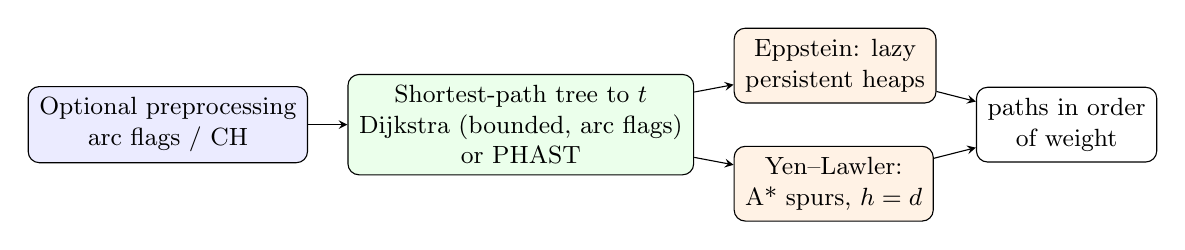
\begin{tikzpicture}[node distance=0.55cm and 0.5cm, every node/.style={font=\small},
  box/.style={draw,rounded corners,align=center,minimum height=0.9cm,inner sep=4pt,fill=#1},
  box/.default=white, ->, >=stealth]
  \node[box=blue!8] (pre) {Optional preprocessing\\ arc flags / CH};
  \node[box=green!8, right=of pre] (tree) {Shortest-path tree to $t$\\ Dijkstra (bounded, arc flags)\\ or PHAST};
  \node[box=orange!10, right=of tree, yshift=0.75cm] (epp) {Eppstein: lazy\\ persistent heaps};
  \node[box=orange!10, right=of tree, yshift=-0.75cm] (yen) {Yen--Lawler:\\ A* spurs, $h=d$};
  \node[box, right=of epp, yshift=-0.75cm] (out) {paths in order\\ of weight};
  \draw (pre) -- (tree); \draw (tree) -- (epp); \draw (tree) -- (yen);
  \draw (epp) -- (out); \draw (yen) -- (out);
\end{tikzpicture}
\caption{A query. The tree supplies the distances $d(v)$ to the goal, which Eppstein uses for the sidetrack deltas and
Yen--Lawler as exact A* lower bounds. The detour bound limits the tree, the enumeration and the spur searches.}
\label{fig:pipeline}
\end{figure}

\subsection{Definitions}\label{sec:definitions}
A directed graph $G=(V,E)$ has $n$ vertices and $m$ edges. An edge $e=(u,v)$ leads from its \emph{tail} $u$ to its
\emph{head} $v$ and has a weight $w(e)\ge 0$; several edges may connect the same two vertices. A \emph{walk} from $s$
to $t$ is a sequence of edges in which each edge starts where the previous one ends; its weight is the sum of its
edge weights. A walk may visit a vertex several times. A walk that visits no vertex twice is a \emph{simple path}.
We say ``path'' for both where the difference does not matter. The \emph{distance} $d(u,v)$ is the smallest weight of
a walk from $u$ to $v$, and infinite if there is none. Given $s$, $t$ and $k$, the \emph{$k$ shortest paths problem}
asks for $k$ walks from $s$ to $t$ of smallest weight, in order of weight; the \emph{$k$ shortest simple paths
problem} asks the same for simple paths. If a graph has a cycle that can be reached from $s$ and from which $t$ can
be reached, it has infinitely many walks from $s$ to $t$ but only finitely many simple paths.

\subsection{Dijkstra's algorithm and the shortest-path tree}\label{sec:dijkstra}
All algorithms below start from the distances of all vertices \emph{to the goal}: $d(v)=d(v,t)$.
Dijkstra's algorithm~\cite{dijkstra1959} computes them. It keeps a tentative distance for every vertex, initially
$0$ for $t$ and infinite for all others, and a priority queue of vertices ordered by tentative distance. It
repeatedly removes the vertex $v$ with the smallest tentative distance, which is then final (\emph{settled}), and
\emph{relaxes} every edge $(u,v)$ entering $v$: if $w(u,v)+d(v)$ is smaller than the tentative distance of $u$, it
becomes the new one, and $(u,v)$ is remembered as the \emph{tree edge} of $u$. Because weights are not negative, a
settled distance can never be improved later. Since the search starts at $t$ and follows edges backwards, we call it
a \emph{backward} search. With a binary heap as priority queue it takes $O((n+m)\log n)$ time.

The tree edges form the \emph{shortest-path tree} $T$: every vertex that can reach $t$ has exactly one tree edge,
to a vertex we call $\mathrm{next}(v)$, and following tree edges from any vertex leads to $t$ along a shortest path.
An edge $(u,v)$ is \emph{tight} if $d(u)=w(u,v)+d(v)$, \ie{} if it lies on some shortest path to $t$; tree edges are
tight, and for every edge $d(u)\le w(u,v)+d(v)$.

\subsection{Eppstein's algorithm: paths as sequences of sidetracks}\label{sec:eppstein}

\begin{figure}[t]
\centering
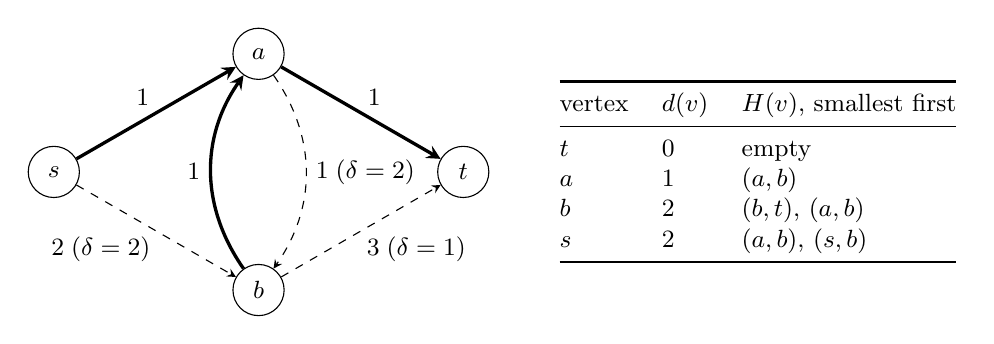
\begin{tikzpicture}[>=stealth, every node/.style={font=\small}, v/.style={circle,draw,minimum size=6.5mm,inner sep=0pt}]
  \node[v] (s) at (0,0) {$s$};
  \node[v] (a) at (2.6,1.5) {$a$};
  \node[v] (b) at (2.6,-1.5) {$b$};
  \node[v] (t) at (5.2,0) {$t$};
  \draw[->,very thick] (s) -- node[above left=-2pt] {1} (a);
  \draw[->,very thick] (a) -- node[above right=-2pt] {1} (t);
  \draw[->,very thick] (b) to[bend left=35] node[left] {1} (a);
  \draw[->,dashed] (a) to[bend left=35] node[right] {1\;($\delta=2$)} (b);
  \draw[->,dashed] (s) -- node[below left=-2pt] {2\;($\delta=2$)} (b);
  \draw[->,dashed] (b) -- node[below right=-2pt] {3\;($\delta=1$)} (t);
  \node[anchor=west,align=left] at (6.3,0) {\begin{tabular}{@{}lll@{}}
    \toprule vertex & $d(v)$ & $H(v)$, smallest first \\ \midrule
    $t$ & 0 & empty \\
    $a$ & 1 & $(a,b)$ \\
    $b$ & 2 & $(b,t)$, $(a,b)$ \\
    $s$ & 2 & $(a,b)$, $(s,b)$ \\ \bottomrule
  \end{tabular}};
\end{tikzpicture}

\medskip
\begin{tabular}{@{}rlll@{}}
\toprule
 & sidetrack sequence & walk & weight \\
\midrule
1 & (none) & $s\,a\,t$ & $2$ \\
2 & $(a,b)$ & $s\,a\,b\,a\,t$ & $2+2=4$ \\
3 & $(s,b)$ & $s\,b\,a\,t$ & $2+2=4$ \\
4 & $(s,b),(b,t)$ & $s\,b\,t$ & $2+2+1=5$ \\
5 & $(a,b),(b,t)$ & $s\,a\,b\,t$ & $2+2+1=5$ \\
6 & $(s,b),(a,b)$ & $s\,b\,a\,b\,a\,t$ & $2+2+2=6$ \\
\bottomrule
\end{tabular}
\caption{Example. Thick edges: the shortest-path tree to $t$; dashed edges: sidetracks with their deltas. $H(v)$
contains the sidetracks that leave the tree path from $v$ to $t$. Below: the six shortest walks and the sidetracks
that describe them. The graph has a cycle ($a\to b\to a$), so there are infinitely many walks.}
\label{fig:example}
\end{figure}

\paragraph{Sidetracks.} Fix the tree $T$ to the goal $t$. An edge $e=(u,v)$ that is not a tree edge is called a
\emph{sidetrack}. Its \emph{delta}
\[\delta(e)=w(e)+d(v)-d(u)\;\ge 0\]
is the extra weight of leaving $u$ over $e$ and continuing optimally, compared with the shortest path from $u$. Take
any walk from $s$ to $t$ and add up the deltas of all its edges (tree edges have delta $0$): the distances cancel
in pairs, and the sum is the weight of the walk minus $d(s)$. Hence
\[\text{weight of a walk}=d(s)+\sum_{\text{its sidetracks }e}\delta(e).\]
A walk is also determined by its sequence of sidetracks alone: between two sidetracks, and after the last one, it
has no choice but to follow tree edges. In \cref{fig:example}, the sidetrack sequence $(s,b),(b,t)$ means: take
$(s,b)$, then, standing at $b$, immediately take $(b,t)$; its weight is $d(s)+2+1=5$. Not every sequence is valid:
after a sidetrack with head $v$, the next sidetrack must start at a vertex on the tree path from $v$ to $t$. So
the problem becomes: \emph{enumerate the valid sidetrack sequences in order of their sum of deltas.} The empty
sequence is the shortest path.

\paragraph{The heaps $H(v)$.} For a vertex $v$, let $H(v)$ be the set of sidetracks whose tail lies on the tree path
from $v$ to $t$; these are exactly the sidetracks that may follow a sidetrack with head $v$ (and $H(s)$ contains
the possible first sidetracks). To find the best ones quickly, $H(v)$ is stored as a \emph{heap}: a binary tree
whose nodes hold one sidetrack each, such that the delta of a node is never larger than the deltas of its children.
The smallest element is at the root, and everything below a node is at least as large as the node.

Storing each $H(v)$ separately would need far too much space, since $H(v)$ consists of the sidetracks leaving $v$
itself plus all of $H(\mathrm{next}(v))$. Eppstein's key idea is to let the heaps share nodes: $H(v)$ is built from
$H(\mathrm{next}(v))$ by adding the sidetracks of $v$ \emph{without changing} $H(\mathrm{next}(v))$, which other
vertices still use. A data structure whose old versions stay valid after an update is called
\emph{persistent}~\cite{driscoll1989}. Here it is obtained by copying the few nodes an update would change instead
of overwriting them.

\paragraph{Enumeration.} A \emph{candidate} is a sidetrack sequence. The algorithm keeps a priority queue of
candidates ordered by weight, starting with the empty sequence, and repeats: remove the lightest candidate,
output it as the next path, and insert its \emph{successors}. For a candidate whose last sidetrack $e$ was taken from
a node $x$ of the heap $H(v)$, the successors are
\begin{itemize}
  \item \emph{replace:} the same sequence with $e$ replaced by the sidetrack of a child of $x$ in the heap (at most
        two successors), and
  \item \emph{append:} the sequence extended by the root of $H(\mathrm{head}(e))$, the best sidetrack that can
        follow $e$ (at most one successor).
\end{itemize}
The empty sequence has one successor, the root of $H(s)$. Two facts make this correct. A successor is never lighter
than its candidate, because a heap child is not smaller than its parent and deltas are not negative; so when a
candidate is removed from the queue, no lighter one can appear later. And every valid sequence is generated exactly
once: its last sidetrack is one node of the heap that belongs to the sequence before it, and there is exactly one
way down from the root of that heap to this node. In the example, the candidate $(a,b)$, the root of $H(s)$,
produces $(s,b)$ by replacement and $(a,b),(b,t)$ by appending the root of $H(b)$, the heap at the head of
$(a,b)$. Each output costs one removal and
at most three insertions, so producing the $k$ lightest sequences takes $O(k\log k)$ time after the tree and the
heaps exist. The graph whose vertices are the heap nodes and whose edges are these successor relations is
Eppstein's \emph{path graph}; with all heaps built in advance in a refined way, his algorithm takes
$O(m+n\log n+k\log k)$ time in total~\cite{eppstein1998}.

\paragraph{In the library: lazy heaps with leftist merging.}
Building the heaps of all vertices in advance is wasteful when only a few paths are requested. Jiménez and
Marzal~\cite{jimenez2003} build $H(v)$ only when the enumeration first needs it, and we follow them: $H(v)$ is
requested for $v=s$ and for the heads of sidetracks of extracted candidates; if $H(\mathrm{next}(v))$ does not exist
yet, it is built first. The library does this iteratively, from the first vertex on the tree path that already has
a heap back towards $v$, so long tree paths cause no deep recursion. The first candidate therefore needs the
heaps of all vertices on the tree path from $s$ to $t$.

For the heaps we use \emph{leftist heaps}~\cite{crane1972}. The \emph{rank} of a node is the number of nodes on the
path that always goes to the right child, down to a missing child. A heap is leftist if at every node the rank
of the left child is at least the rank of the right child; then the rightmost path of a heap with $N$ nodes has at
most $\log_2(N+1)$ nodes. Two leftist heaps are \emph{merged} by comparing the roots, keeping the smaller one as the
new root, merging its right subtree with the other heap in the same way, and finally swapping the two children if
the right one has the larger rank. Only nodes on the two rightmost paths are touched. For persistence, the merge
writes each touched node as a new copy and leaves the old one unchanged, so both input heaps remain valid and the
result shares all untouched nodes with them. Eppstein keeps the sidetracks of each vertex in a small heap of their
own and inserts only its root into a balanced heap along the tree path. We simplify this: the sidetracks leaving
$v$ are sorted by delta and linked into a chain through their left children (a valid leftist heap whose rightmost
path has length one), and this chain is merged into $H(\mathrm{next}(v))$. The merge copies $O(\log m)$ nodes, so
$H(v)$ costs $O(\deg(v)\log\deg(v)+\log m)$ time and $O(\log m)$ additional nodes.

A candidate is stored as a pointer to its parent candidate and one heap node, so creating one costs $O(1)$, and its
weight is the weight of the sequence it extends plus one delta. To output a path as a list
of edges, the library collects the sidetracks by following the parent pointers and then walks from $s$ to $t$,
taking the next sidetrack where its tail is reached and tree edges otherwise. This costs time proportional to the
length of the path and dominates in practice (\cref{tab:enumeration}); an iterator that returns only the weights
skips it.

\subsection{Detour bound (``corridor'')}\label{sec:corridor}
Users rarely want arbitrarily long alternatives. With an absolute or relative detour limit $\Delta$, only paths of
weight at most $d(s)+\Delta$ are admissible; enumerating them is known as the near-shortest paths
problem~\cite{byers1984,carlyle2005}. The bound prunes all three stages of a query. A vertex $v$ with
$d(v)>d(s)+\Delta$ cannot lie on an admissible path, so the backward Dijkstra stops as soon as it would settle a
vertex beyond the radius $d(s)+\Delta$ (the radius becomes known when $s$ is settled, which happens before any
vertex farther away than $s$ is settled). In the enumeration, a candidate with $\sum\delta>\Delta$ is not inserted
into the queue, and since successors are never lighter, nothing is lost. The A* spur searches of
\cref{sec:yen} stop in the same way. The library calls this the \emph{corridor}. Two remarks put it into
perspective. First, the region that is searched is a ball around $t$, not an ellipse around the $s$--$t$
path: the exact condition for a vertex is $d(s,v)+d(v)\le d(s)+\Delta$, which needs forward distances from $s$ as
well. A bidirectional search, or K*~\cite{aljazzar2011}, which builds the path graph while an A* search explores the
graph, would search a smaller region; our bound is simply the part that a single backward search gives for free. It
helps when $s$ and $t$ are close relative to the size of the graph, and not at all when they are far apart. Second,
with the bound the number of admissible paths is finite even with cycles, provided that no cycle of weight zero
lies on an admissible walk; a query can then be iterated to its end.

\subsection{Simple paths: Yen's algorithm with Lawler's rule and A*}\label{sec:yen}
In networks with two-way edges most of the shortest walks are the shortest path plus a small loop (in
\cref{fig:example}, walks 2 and 6), not real alternatives. With \texttt{SimplePathsOnly}, the library returns
simple paths only, using a different algorithm, since no way is known to restrict Eppstein's path graph to simple
paths without checking each walk.

\paragraph{Yen's algorithm.} The first path $P_1$ is the shortest path, which is simple. Every other simple path
$Q$ from $s$ to $t$ \emph{deviates} from each previously found path somewhere. Yen's algorithm~\cite{yen1971} uses
this to derive new paths from found ones. Let $P=(v_0=s,v_1,\dots,v_\ell=t)$ be a path that has just been output.
For each position $i<\ell$, the prefix $(v_0,\dots,v_i)$ is called the \emph{root} and $v_i$ the \emph{spur vertex}.
The algorithm computes the shortest path from $v_i$ to $t$, the \emph{spur}, in a restricted graph in which
\begin{itemize}
  \item the vertices $v_0,\dots,v_{i-1}$ of the root are removed, so that root plus spur is simple, and
  \item every edge leaving $v_i$ that some already found path with the same root uses next is removed, so that the
        result differs from all found paths.
\end{itemize}
Root plus spur is the best simple path that shares exactly this root with $P$ and then leaves it, and it becomes
a \emph{candidate}. The next path to output is the lightest candidate found so far, kept in a priority queue.
The algorithm is correct because the next simple path, whatever it is, shares some root with a found path and
then leaves all found paths with that root, so it is the best path of one of the restricted problems that have been
solved. Each output path causes up to $n$ shortest-path computations, which gives $O(kn(m+n\log n))$ time in the
worst case.

\paragraph{Lawler's rule.} Every path except $P_1$ was created as a candidate from a parent path at some position
$j$, its \emph{deviation index}: up to $v_j$ it equals its parent. Lawler~\cite{lawler1972} observed that for
positions $i<j$ the restricted problem is the same one that was already solved when the parent was processed: the
root is the same, and the new path adds no removed edge there, because at $v_i$ it uses the same edge as its
parent. Only positions $i\ge j$ need spur computations. This removes duplicate candidates and many searches.

\paragraph{A* with exact distances.} A spur is a point-to-point shortest path, for which Dijkstra's algorithm
explores much more of the graph than necessary. A* search~\cite{hart1968} runs forward from the spur vertex and
orders its priority queue by $g(v)+h(v)$, where $g(v)$ is the tentative distance from the spur vertex and $h(v)$ a
lower bound (\emph{potential}) on the remaining distance to $t$. If $h(u)\le w(u,v)+h(v)$ holds for all edges
(\emph{consistency}), every vertex is settled at most once and the search may stop when $t$ is settled. The better
the bound, the fewer vertices are explored. Here an excellent bound is available for free: the distances $d(v)$ of
the shortest-path tree of the unrestricted graph. Removing vertices and edges can only make distances longer, so
$d$ is a lower bound in every restricted graph, and it is consistent (\cref{sec:dijkstra}). When the tree path from
the spur vertex survives the restrictions, the search settles only the vertices of that path; otherwise it explores
only where the restrictions force a detour.

\paragraph{In the library.} The found paths are stored in a trie (a tree in which each path from the root spells
the edge sequence of a prefix); the edges to remove at a spur vertex are the children of the root's trie node. The
tree to $t$ is computed once per query, as for Eppstein. Spurs of a path are generated lazily when the next path
is requested, so asking for one path costs no spur search. With a detour bound, a spur search stops as soon as the
smallest $g+h$ in its queue exceeds what an admissible path may still cost. Using the reverse tree to guide or avoid
spur searches is known~\cite{feng2014,kurz2016}; we do not yet skip the search when the tree path itself is a
valid spur, which those algorithms do.

\subsection{Arc flags}\label{sec:arcflags}
The remaining techniques invest preprocessing time to make the shortest-path tree of later queries cheaper. For
\emph{arc flags}~\cite{lauther2004,moehring2006}, the vertices are partitioned into a small number of
\emph{regions}. Every edge gets one bit per region; the bit of edge $e$ for region $R$ is set if $e$ lies on a
shortest path to some vertex of $R$. A search for a goal in region $R$ may then ignore all edges whose bit for $R$
is not set, because no shortest path to the goal uses them.

The bits are computed as follows. An edge inside $R$ gets the bit for $R$. A shortest path that enters $R$ from
outside must pass through a \emph{boundary vertex} of $R$, a vertex of $R$ with an incoming edge from another
region, and up to that vertex it is a shortest path to the boundary vertex. So for every boundary vertex $b$ of $R$,
one backward Dijkstra from $b$ computes the distances to $b$, and every edge that is tight for these distances
gets the bit for $R$. The preprocessing costs one Dijkstra run per boundary vertex, which is why partitions with
few boundary vertices matter.

\paragraph{In the library.} The partition comes from chunks of a breadth-first order (built in), from a string, or
from an external partitioner such as Mt-KaHyPar~\cite{mtkahypar}, for which the library writes the METIS input
format. The backward Dijkstra of a query relaxes only edges flagged for the goal's region. Every vertex still gets
its correct distance, because its shortest path to $t$ consists of flagged edges. But since Eppstein needs the
distance of \emph{every} vertex that can reach the goal, arc flags cannot skip vertices here, as they do in a
point-to-point query; they only skip edge relaxations, so the gain is small by construction (\cref{tab:ch}). The
documentation recommends the detour bound first.

\subsection{Contraction hierarchy and PHAST}\label{sec:ch}

\paragraph{Contraction.} A \emph{contraction hierarchy} (CH)~\cite{geisberger2008} removes the vertices from the graph
one by one. To \emph{contract} a vertex $v$ means to remove it while preserving all distances between the remaining
vertices: for every remaining in-neighbor $u$ and out-neighbor $x$ of $v$, if the path $u\to v\to x$ is the only
shortest path from $u$ to $x$, a \emph{shortcut} edge $(u,x)$ with weight $w(u,v)+w(v,x)$ is added. Whether another
path of at most that weight exists is decided by a \emph{witness search}, a Dijkstra search from $u$ that avoids
$v$. It may be cut off after a fixed number of settled vertices; if it then has found no witness, the shortcut is
added anyway, which costs space but never correctness. The order of contraction defines the \emph{rank} of each
vertex. A good order contracts unimportant vertices first and keeps the number of shortcuts small; the usual
heuristic picks the vertex with the smallest \emph{edge difference} (shortcuts added minus edges removed) next.

Let $G^+$ be the original graph plus all shortcuts. Call an edge \emph{upward} if it leads to a vertex of higher
rank and \emph{downward} otherwise. The construction guarantees that for any two vertices $u$ and $t$ with a path
between them, $G^+$ contains a shortest path from $u$ to $t$ that first uses only upward edges and then only
downward edges (an \emph{up--down path}): wherever a shortest path has a vertex that is lower than both its
neighbors on the path, that vertex was contracted before them, and either a shortcut or a witness path replaces
the dip. A point-to-point query exploits this with two small searches, one upward from each end.

\paragraph{PHAST.} Eppstein needs the distances of all vertices to $t$, not one. PHAST~\cite{delling2013phast}
computes them from the hierarchy in two phases.
\begin{enumerate}
  \item \emph{Upward search from $t$.} A backward Dijkstra from $t$ that follows only downward edges, backwards. It
        reaches only vertices of higher rank than $t$, typically a few hundred, and gives each of them the length of
        the best purely downward path to $t$.
  \item \emph{Sweep.} All vertices are processed once, in order of descending rank. For each vertex $u$, every
        upward edge $(u,x)$ is relaxed: $d(u)\leftarrow\min(d(u),w(u,x)+d(x))$.
\end{enumerate}
After the sweep every $d(u)$ is correct, by induction over the rank: the shortest up--down path from $u$ is either
purely downward, and was found in phase 1, or it starts with an upward edge $(u,x)$ and continues with a shortest
up--down path from $x$, whose distance is already final because $x$ has a higher rank and was processed earlier. The
sweep needs no priority queue and reads memory in a fixed order, which is why it is much faster than Dijkstra's
algorithm on graphs with a good hierarchy. RPHAST~\cite{delling2011rphast} restricts the sweep to the vertices that
matter for a given set of targets, and customizable contraction hierarchies~\cite{dibbelt2016} separate an order
that depends only on the graph's structure from a fast update for new weights.

\paragraph{In the library.} The contraction order is maintained lazily (a vertex's priority is recomputed when it
reaches the front of the queue) by edge difference plus the number of already contracted neighbors, which spreads
the contraction evenly; witness searches have a settled-vertex limit, and of parallel edges only the lightest is
kept. Vertices are stored in sweep order. Eppstein also needs the tree, not only the distances. Unpacking shortcuts
is unnecessary: we rebuild the tree from the \emph{original} edges that are tight, breadth-first from $t$. Choosing an
arbitrary tight edge per vertex would be wrong if the graph has cycles of weight zero, because the chosen edges
could close such a cycle; the breadth-first order prevents this. This pass over all edges is part of the PHAST
times we report. With a detour bound the bounded Dijkstra usually visits fewer vertices than PHAST and is used
instead. For Yen--Lawler the hierarchy accelerates only the one initial tree, not the spur searches. To our
knowledge, the combination of Eppstein's enumeration with PHAST has not been described before; a point-to-point CH
query would not be enough for it.

\subsection{Data layout and exactness}
Vertices and edges are stored in flat arrays (structure of arrays): tail, head, weight and group per edge, and
compressed adjacency rows by direction, rebuilt lazily after a change. Per-vertex query data (distance, tree edge,
heap root) live in arrays that are reused across queries: a vertex's entry is valid only if its \emph{stamp} equals
the current query number, so a query touches only the vertices it reaches and never resets the arrays. Public
\texttt{Vertex}, \texttt{Edge} and \texttt{Path} types are small values that refer to these arrays. Weights are
64-bit integers; an edge with a negative weight is treated as switched off. All techniques keep the results exact:
the same paths with the same weights are returned with and without a detour bound (up to the bound), arc flags and
the hierarchy; only paths of equal weight may come in a different order.

\section{Related work}\label{sec:related}

The previous section introduced the algorithms we build on; here we place them among the alternatives.

\paragraph{Paths that may repeat vertices.} Eppstein's algorithm~\cite{eppstein1998} is the reference for walks.
Jiménez and Marzal proposed the recursive enumeration algorithm~\cite{jimenez1999}, which computes the $k$-th path
to a vertex from the paths to its predecessors, and later the lazy version of Eppstein's
algorithm~\cite{jimenez2003} that we use; both are faster in practice than the original. K*~\cite{aljazzar2011}
interleaves an A* search with the construction of the path graph, so that the full tree is never needed.

\paragraph{Simple paths.} Beyond Yen~\cite{yen1971} and Lawler~\cite{lawler1972}, much work reduces the cost of the
spur searches: Hershberger et al.~\cite{hershberger2007} use replacement paths, Feng~\cite{feng2014} uses the
reverse shortest-path tree to restrict each search to the vertices that can matter, and Kurz and
Mutzel~\cite{kurz2016} and Al Zoobi et al.~\cite{alzoobi2023} combine Eppstein's sidetrack idea with simplicity
checks and avoid many spur searches altogether. Alternative routes~\cite{abraham2013} and $k$ shortest paths with
limited overlap~\cite{chondrogiannis2020} address a related problem, where paths must be sufficiently different.

\paragraph{Speed-up techniques.} Arc flags and contraction hierarchies are two of many techniques for route
planning in road networks; Bast et al.~\cite{bast2016} give a survey.

\paragraph{Languages, garbage collection and measurement.}
Hertz and Berger~\cite{hertz2005} quantified that garbage collection can match explicit memory management in speed
if it is given several times more memory. Comparisons of the same program in several
languages~\cite{prechelt2000,hundt2011} show that the differences between implementations within one language are
often as large as those between languages, which is a caveat for our single implementation per language. For
runtimes with JIT compilers, start-up and steady state must be separated, and steady state is not always
reached~\cite{georges2007,barrett2017}; an earlier version of our own measurements illustrates the problem
(\cref{sec:discussion}).

\section{Three implementations}\label{sec:languages}

\Cref{tab:loc} summarizes the implementations. They follow the same structure file by file; the interfaces differ
only where the languages differ (exceptions vs.\ error values vs.\ \texttt{Result}, properties vs.\ methods,
\texttt{IEnumerable} vs.\ Go iterators vs.\ Rust iterators).

\begin{table}[t]
\centering
\caption{Implementations. Lines exclude blank and comment lines.}
\label{tab:loc}
\begin{tabular}{lrrl}
\toprule
 & library & tests & notable language-specific choices \\
\midrule
2010 original (\cs) & 486 & -- & object graph, sorted-list priority queue \\
\cs{} (.NET 8/10) & \NumLocCs & \NumLocCsTests & \texttt{readonly struct} views, \texttt{PriorityQueue}, FsCheck \\
Go 1.23+ & \NumLocGo & \NumLocGoTests & generic heap, \texttt{iter.Seq}, native fuzzing \\
Rust 2021 & \NumLocRust & \NumLocRustTests & arenas with \texttt{u32} links, borrow-checked iterators \\
\bottomrule
\end{tabular}
\end{table}

\paragraph{Memory management.} The graph and the per-vertex query data are flat arrays in all three languages. The
enumeration differs: in \cs{} and Go, heap nodes and candidates are small objects managed by the garbage collector;
in Rust they live in two vectors (arenas) per query and refer to each other by \texttt{u32} indices, and the arenas
are cleared at the next query. There is no reference counting and no unsafe code in the Rust library. Every returned
path is a freshly allocated list of edges in all three.

\paragraph{Safety of iteration.} All three offer an iterator over the paths of a query. Changing the graph during the
iteration is a runtime error in \cs{} (\texttt{InvalidOperationException}) and Go (panic). In Rust the iterator
borrows the graph mutably, so the same mistake is a compile-time error; reading the graph during the iteration goes
through the iterator.

\paragraph{Labels.} Vertex labels are case-insensitive. \cs{} and Go keep the caller's string if it is already in
upper case; the Rust version stores all label text in one string and indexes it with an open-addressing hash table,
which avoids one heap allocation and one map entry per vertex. (A first, straightforward Rust version stored each
label twice and needed 200\,MB instead of 112\,MB for the largest graph.)

\paragraph{Testing.} The three implementations read the same golden files (graphs and expected paths, including
DIMACS input), and compare against brute-force enumeration on thousands of random small graphs with cycles, zero
and negative weights, detour bounds, arc flags and contraction hierarchies. \cs{} adds property-based tests
(FsCheck), Go adds coverage-guided fuzzing of the importers and of the path enumeration. CI enforces coverage gates
(\cs{} $\ge 95\%$ lines, Go $\ge 93\%$ statements); the Rust tests are the smallest suite and have no coverage gate.

\section{Experiments}\label{sec:experiments}

\paragraph{Setup.} All measurements ran on \NumCpu{} (4 virtual cores, Linux) with .NET~\NumDotnet, \NumGo{} and
rustc~\NumRustc{} (release builds; Rust with one codegen unit). The benchmark is the same program in the three
languages. It builds a $n\times n$ grid (vertex $v=y\,n+x$; edges to the right and lower neighbor, and every tenth
vertex also to its left neighbor, which creates cycles); \texttt{two-way} grids have every street in both directions.
Weights are $1+(r \bmod 100)$ for $r$ drawn from SplitMix64~\cite{steele2014} with seed 1, implemented identically
in all three languages, so all of them build exactly the same graphs. The benchmark prints the weight of the last
path, and the measurement script aborts if the languages disagree; they agreed in every scenario.

\paragraph{What is measured.} Each scenario ran in a fresh process \NumRepeat{} times per language (once where a
table says so); we report the median over the processes. Inside a process, the query is issued 22 times. The
\emph{first} query includes one-time work (adjacency rows, JIT compilation). The \emph{second} is what a short
benchmark would report. The \emph{steady-state} time is the median of the 20 further identical queries; it is the
time of the shortest-path tree plus the first path, and is what the tables call ``tree''. Separating the
three matters for JIT-compiled runtimes~\cite{georges2007,barrett2017} and changes the conclusions
(\cref{sec:discussion}). ``Next'' is the time for the remaining $k-1$ paths, measured once per process after the
last of these queries. The benchmark also records the garbage collections, their total pause time and the bytes
allocated during ``next'' (from the runtimes' own counters; in Rust from a counting allocator), the live heap after
the first query, and the script records the peak resident memory of the process. As a measure of dispersion we
computed, for every time of at least 1\,ms, the range (largest minus smallest value over the \NumRepeat{}
processes) relative to the median: its median over all entries is \NumSpreadMedian\%, its 90th percentile
\NumSpreadNinety\% and its maximum \NumSpreadMax\%. Differences between languages below roughly
\NumSpreadNinety\% should therefore not be interpreted.

\begin{table}[t]
\centering
\caption{Eppstein, corner to corner on one-way grids (median times in ms). Tree: repeated query; next: the remaining $k-1$ paths. Fastest per group in bold (within 3\%).}
\label{tab:eppstein}
\small
\begin{tabular}{lrrrrrr}
\toprule
 & \multicolumn{3}{c}{tree} & \multicolumn{3}{c}{next paths} \\ \cmidrule(lr){2-4}\cmidrule(lr){5-7}
 & \cs{} & Go & Rust & \cs{} & Go & Rust \\
\midrule
$200^2$, $k=10^4$ & 29.2 & 8.6 & \textbf{7.3} & 79.6 & 45.5 & \textbf{35.3} \\
$500^2$, $k=10^4$ & 54.0 & 73.4 & \textbf{52.4} & \num{205} & \num{113} & \textbf{88.6} \\
$1000^2$, $k=10^4$ & \textbf{\num{255}} & \num{312} & \textbf{\num{260}} & \num{406} & \num{359} & \textbf{\num{314}} \\
$1000^2$, $k=10^5$ & \textbf{\num{253}} & \num{331} & \num{272} & \num{3419} & \num{3436} & \textbf{\num{3079}} \\
\bottomrule
\end{tabular}
\end{table}

\begin{table}[t]
\centering
\caption{Enumerating $10^5$ paths on the $10^6$-vertex grid after the tree is known: time with and without writing out the paths, and the memory allocated and garbage collections during the enumeration with paths.}
\label{tab:enumeration}
\small
\begin{tabular}{lrrr}
\toprule
 & \cs{} & Go & Rust \\
\midrule
paths written out (ms) & \num{3094} & \num{3188} & \textbf{\num{2804}} \\
weights only (ms) & \num{144} & 44.4 & \textbf{28.4} \\
\midrule
allocated, paths written out (MB) & 839 & 855 & 837 \\
garbage collections & 6 & 5 & -- \\
total GC pause (ms) & 119.6 & 0.5 & -- \\
allocated, weights only (MB) & 32 & 37 & 15 \\
\bottomrule
\end{tabular}
\end{table}


\paragraph{Eppstein, corner to corner (\cref{tab:eppstein,tab:enumeration}).} Grids with $4\cdot10^4$ to $10^6$
vertices, paths across the whole graph. EPPSTEINTEXT

\begin{table}[t]
\centering
\caption{Nearby vertices in the middle of the $10^6$-vertex grid, $k=10^4$ (ms). First: first query (includes one-time work such as JIT compilation and building adjacency rows).}
\label{tab:local}
\small
\begin{tabular}{lrrrrrrrrr}
\toprule
 & \multicolumn{3}{c}{first query} & \multicolumn{3}{c}{tree} & \multicolumn{3}{c}{next paths} \\ \cmidrule(lr){2-4}\cmidrule(lr){5-7}\cmidrule(lr){8-10}
 & \cs{} & Go & Rust & \cs{} & Go & Rust & \cs{} & Go & Rust \\
\midrule
no corridor & \num{218} & \num{115} & \textbf{98.0} & \textbf{65.5} & 84.4 & 69.1 & 33.3 & \textbf{10.5} & \textbf{10.7} \\
\texttt{MaxDetourRatio} $=0.1$ & 46.8 & \textbf{21.6} & 27.5 & 3.0 & 0.80 & \textbf{0.50} & 32.0 & \textbf{10.7} & \textbf{11.0} \\
\bottomrule
\end{tabular}
\end{table}


\paragraph{Detour bound (\cref{tab:local}).} Two vertices in the middle of the $10^6$-vertex grid, 50 columns and 50
rows apart. Without a bound, the tree covers every vertex that can reach the goal; with paths limited to 10\% above
the shortest one, it covers only a neighborhood of the goal. LOCALTEXT

\begin{table}[t]
\centering
\caption{Building the $10^6$-vertex grid ($2.1\cdot10^6$ edges), in ms; live memory of the graph with one query and peak resident memory of the whole benchmark process (built by index, $k=10^4$).}
\label{tab:build}
\small
\begin{tabular}{lrrr}
\toprule
 & \cs{} & Go & Rust \\
\midrule
by index & \num{460} & \num{661} & \textbf{\num{279}} \\
by label strings & \num{1326} & \num{1175} & \textbf{\num{863}} \\
DIMACS text import & \num{704} & \num{1020} & \textbf{\num{473}} \\
\midrule
live memory of the graph (MB) & 84 & 94 & 112 \\
peak resident memory of the process (MB) & 406 & 344 & 220 \\
\bottomrule
\end{tabular}
\end{table}


\begin{table}[t]
\centering
\caption{Simple paths (Yen--Lawler with A*) on two-way grids: time for the paths after the first (ms).}
\label{tab:yen}
\small
\begin{tabular}{lrrr}
\toprule
 & \cs{} & Go & Rust \\
\midrule
$200^2$, $k=100$ & \num{864} & \num{930} & \textbf{\num{666}} \\
$200^2$, $k=1000$ & \textbf{\num{5512}} & \num{7402} & \num{5773} \\
$1000^2$ local, ratio 0.1, $k=100$ & 95.7 & 50.9 & \textbf{34.5} \\
\bottomrule
\end{tabular}
\end{table}


\paragraph{Simple paths (\cref{tab:yen}).} Two-way grids, where simple paths matter. YENTEXT

\begin{table}[t]
\centering
\caption{Preprocessing techniques: preprocessing time and the steady-state shortest-path tree, in ms, and the number of shortcuts (Rust; \cs{} differs slightly because of tie-breaking). The 16-region arc flags and the $1000^2$ contraction were run in one process per language.}
\label{tab:ch}
\small
\begin{tabular}{lrrrrrrr}
\toprule
 & \multicolumn{3}{c}{preprocessing} & \multicolumn{3}{c}{tree (steady state)} \\ \cmidrule(lr){2-4}\cmidrule(lr){5-7}
 & \cs{} & Go & Rust & \cs{} & Go & Rust & shortcuts \\
\midrule
$200^2$ two-way: Dijkstra & -- & -- & -- & \textbf{7.9} & 10.5 & 9.3 & -- \\
\quad arc flags, 4 regions & \num{11.2}\,s & \num{12.6}\,s & \textbf{\num{10.3}\,s} & \textbf{6.8} & 8.6 & 7.4 & -- \\
\quad arc flags, 16 regions & \textbf{\num{45.3}\,s} & \num{52.7}\,s & \textbf{\num{45.3}\,s} & \textbf{6.7} & 7.9 & \textbf{6.9} & -- \\
\quad CH + PHAST & \num{3008} & \num{2793} & \textbf{\num{2501}} & 3.7 & 3.1 & \textbf{2.3} & 179{,}980 \\
\midrule
$1000^2$ one-way: Dijkstra & -- & -- & -- & \textbf{\num{260}} & \num{316} & \num{273} & -- \\
\quad CH + PHAST & \num{79.2}\,s & \num{70.9}\,s & \textbf{\num{65.8}\,s} & \num{107} & 87.5 & \textbf{81.5} & 3{,}051{,}496 \\
\bottomrule
\end{tabular}
\end{table}


\paragraph{Arc flags and contraction hierarchy (\cref{tab:ch}).} CHTEXT

\begin{figure}[t]
\centering
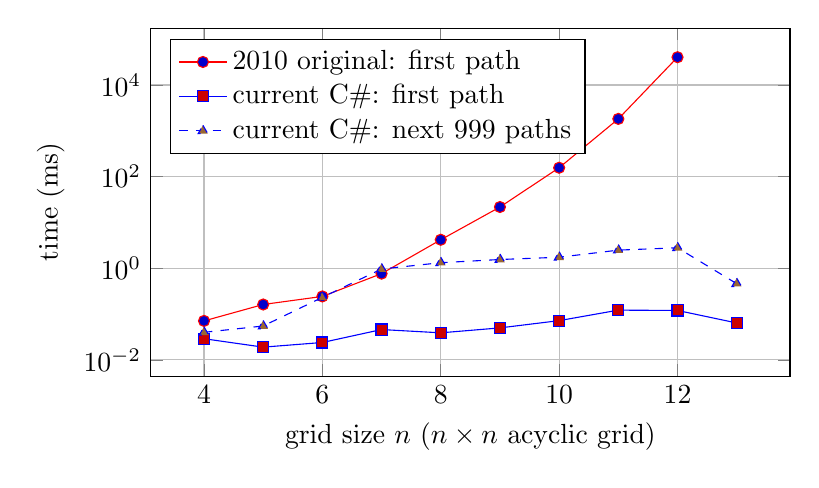
\begin{tikzpicture}
\begin{semilogyaxis}[width=0.8\textwidth,height=6cm,xlabel={grid size $n$ ($n\times n$ acyclic grid)},
  ylabel={time (ms)},legend pos=north west,grid=major,legend cell align=left]
\addplot+[mark=*,red] coordinates {(4,0.071) (5,0.162) (6,0.243) (7,0.764) (8,4.189) (9,21.712) (10,156.248) (11,1820.357) (12,40345.372)};
\addlegendentry{2010 original: first path}
\addplot+[mark=square*,blue] coordinates {(4,0.029) (5,0.019) (6,0.024) (7,0.046) (8,0.039) (9,0.05) (10,0.072) (11,0.122) (12,0.12) (13,0.064)};
\addlegendentry{current \cs{}: first path}
\addplot+[mark=triangle*,blue,dashed] coordinates {(4,0.04) (5,0.055) (6,0.232) (7,0.964) (8,1.323) (9,1.553) (10,1.741) (11,2.489) (12,2.797) (13,0.461)};
\addlegendentry{current \cs{}: next 999 paths}
\end{semilogyaxis}
\end{tikzpicture}
\caption{The 2010 implementation enumerates all $\binom{2(n-1)}{n-1}$ paths in the first query; the current one
computes one tree and then each path on demand.}
\label{fig:baseline}
\end{figure}


\paragraph{The 2010 original (\cref{fig:baseline}).} On acyclic grids, where it terminates at all, the original
implementation's first query enumerates every path: 156\,ms for $10\times10$ (48,620 paths), 1.8\,s for $11\times11$
and 40\,s and 132\,MB for $12\times12$ (705,432 paths). The current version needs about 0.1\,ms for the first path
and less than 3\,ms for the next 999, independent of the number of paths in the graph. On graphs with cycles, the
original does not terminate. This comparison shows the difference between an eager prototype and a lazy algorithm,
not a tuning effect; it was measured once, in one process.

\section{Discussion: garbage collection and language}\label{sec:discussion}
\begin{table}[t]
\centering
\caption{Runtime settings (median ms). Turning garbage collection off (Go) or making it rare (\cs{}) has no measurable effect; disabling tiered compilation makes short \cs{} runs 2--4$\times$ faster.}
\label{tab:runtime}
\small
\begin{tabular}{lrrrrrr}
\toprule
 & \multicolumn{2}{c}{Eppstein $200^2$, $k=10^4$} & \multicolumn{2}{c}{Eppstein $1000^2$, $k=10^5$} & \multicolumn{2}{c}{Yen $200^2$, $k=10^3$} \\ \cmidrule(lr){2-3}\cmidrule(lr){4-5}\cmidrule(lr){6-7}
 & tree & next & tree & next & tree & next \\
\midrule
\cs{} default & 27.7 & 76.2 & \num{255} & \num{3441} & 38.1 & \num{5485} \\
\cs{} gen0 budget 256\,MB & 28.5 & 78.9 & \num{257} & \num{3489} & 38.4 & \num{5428} \\
\cs{} without tiered JIT & 6.4 & 42.9 & \num{248} & \num{3332} & 8.6 & \num{5331} \\
Go default & 9.0 & 43.9 & \num{324} & \num{3468} & 10.9 & \num{7581} \\
Go \texttt{GOGC=off} & 8.0 & 42.7 & \num{318} & \num{3451} & 12.4 & \num{7646} \\
Rust & 6.6 & 34.8 & \num{259} & \num{3092} & 9.4 & \num{5869} \\
\bottomrule
\end{tabular}
\end{table}

DISCUSSIONTEXT

\section{AI-assisted development}\label{sec:ai}

\subsection{Process}
The whole project is an experiment with Claude~\cite{claudecode}. The author worked with it as a coding agent in a
cloud development environment with access to the repository. Claude read and wrote the code, ran builds, tests,
benchmarks and a fuzzer, searched the literature, opened pull requests and reacted to CI results; the author decided
what to do next, chose among the options it proposed, and merged. All work happened in \NumSessions{} sessions over
three days (\NumDays); \NumPullRequests{} pull requests were merged before the first version of this paper. The
author's requests were short and informal, usually one sentence, and never a specification.

\subsection{What the human contributed}
Three kinds of input shaped the result. \emph{The old algorithm} fixed the interface (labels, groups,
\texttt{FindShortestPath}/\texttt{FindNextShortestPath}) and the domain; much of the later work kept that interface
or broke it only when the author allowed it. \emph{Open questions} (what would improve the project most, how to make
it much faster, what is missing for a high-quality library) delegated the search for improvements to Claude, while
the author kept the decisions by choosing among the proposed items. \emph{Expert ideas} (arc flags with a real
partitioner, contraction hierarchies, the idea for a paper) came from a colleague's review and redirected the work
towards algorithm engineering. Explicit constraints, such as excluding multithreading or allowing breaking interface
changes, were the most effective requests.

\subsection{What Claude did, and where it failed}
Claude wrote all code, tests, documentation and benchmarks of version~2, ran every measurement in this paper, and
proposed most of the ideas that were implemented. It also argued \emph{against} ideas when its measurements did not
support them: it first advised against contraction hierarchies, because the measured bottleneck of long queries was
the number of spur searches, and after being asked to implement them it reported that the gain on grids
(\NumPhastSpeedupBig$\times$ for the tree) is below the order of magnitude reported for road networks. The failures
in the code were caught by tests, not by review:
\begin{itemize}
  \item Hand-computed expected values in new tests were wrong several times (\eg{} the weights of simple paths in a
        small two-way graph, and the edges of Eppstein's example typed from memory in the Rust tests); in each case
        brute force or the shared golden data showed that the library was right and the expectation wrong.
  \item Fuzzing found that the Go DIMACS importer treated some Unicode white space differently from line splitting,
        and that Claude's own test harness had an $O(n^2)$ sort.
  \item A scripted text edit broke a Go struct tag; the build caught it.
  \item The first Rust port stored labels twice; the cross-language memory comparison exposed it.
  \item The environment could not download the DIMACS road networks (the server is not reachable from it),
        so all experiments use synthetic grids (\cref{sec:limitations}).
\end{itemize}

\subsection{A critical review of the first version of this paper}
The text has no test suite. On the third day the author asked Claude to review the first version of this paper
critically, as a referee would. The review found errors of a different kind than those in the code:
\begin{itemize}
  \item \emph{A wrong citation.} The lazy variant of Eppstein's algorithm was attributed to Jiménez and Marzal's
        1999 paper, which introduces the recursive enumeration algorithm; the lazy variant is their 2003 paper.
        Relevant related work (K*, near-shortest paths, Feng, Hershberger et al.) was missing, which made the
        detour bound and the A* spur searches look more original than they are.
  \item \emph{Claims without data.} The text stated a 20\% gain for arc flags, a ``3--10$\times$'' gain for PHAST
        and that writing out paths dominates the enumeration; none of these had a measurement in the paper. The
        first two were not confirmed as stated (\cref{tab:ch}); the third was (\cref{tab:enumeration}).
  \item \emph{A confounded headline result.} The main table reported the second query of each process as ``the
        tree'' and showed \cs{} 3--4$\times$ slower than Rust on a small grid. The text explained this as JIT
        warm-up, but the table and the abstract's ``Rust is the fastest in most scenarios'' still rested on it. With
        steady-state measurements the ranking changes (\cref{sec:discussion}).
  \item \emph{An indirect argument.} ``Garbage collection is not a factor'' was inferred from wall-clock times with
        the collector disabled, without checking how often it ran or how long it paused, and although disabling a
        collector changes more than the collections.
  \item \emph{Small inaccuracies.} The number of paths within a detour bound was called finite without excluding
        zero-weight cycles, ``allocation-free'' described a layout whose enumeration allocates, and a stated
        maximum gap of 4$\times$ contradicted a 6$\times$ entry in a table of the same paper.
\end{itemize}
All of these read plausibly, and none would have been caught by the tests. They share a pattern with the wrong
expected values above: statements produced from memory or from an explanation that sounded right, where a
measurement or a look at the source was possible. The remedy was the same as for the code. The benchmark programs
now measure what the text claims, and every measured number in the running text is inserted from the data files by
a macro; the statements about the 2010 baseline and about cited work are the exceptions.

\subsection{Observations}
The decisive factor for reliability was the test infrastructure that Claude built early: golden data shared by all
implementations, brute-force oracles and fuzzing. It made large refactorings (object graph to arrays; three
languages) cheap to verify and let the author accept changes without reading every line. Claude was most useful as
an algorithm engineer when asked open questions and given freedom, and most precise when given constraints. It never
needed a formal specification; it needed a way to check itself. Where no such check existed, in the prose of a
paper, it produced confident errors, and found them only when asked explicitly to doubt its own text.

\section{Threats to validity}\label{sec:limitations}
\emph{Inputs.} All experiments use synthetic grids with uniform random weights. They have no hierarchy, which makes
them a hard case for contraction hierarchies, and the one-way grids are almost acyclic. Results on road networks
(DIMACS~\cite{dimacs9}, OpenStreetMap) may differ in both directions; this is the most important missing
experiment. Each scenario uses one graph (one seed) and one $s$--$t$ pair, so the times do not average over queries.

\emph{Measurement.} The machine is a shared cloud VM with unknown neighbors; we report medians of fresh processes
and the dispersion, but no confidence intervals. The contraction of the largest graph and the 2010 baseline were
measured once. The live-heap numbers are measured differently in each language (after a full collection in \cs{} and
Go, allocator bytes in Rust), and peak resident memory includes the benchmark's own edge list.

\emph{Language comparison.} There is one implementation per language, all generated by the same AI model, the Go and
Rust versions as ports. The implementations are not identical in every data structure (objects vs.\ arenas for the
enumeration, a 4-ary vs.\ binary heaps, different hash tables), so differences between languages cannot be attributed
to the garbage collector or the compiler alone, and other programmers would obtain other ratios~\cite{prechelt2000}.
The conclusions hold for single-threaded code with a data layout that avoids allocation in the search loops; they
say nothing about allocation-heavy or concurrent programs.

\emph{Case study.} The case study has a sample size of one author and one AI model. This paper itself, including
the review in \cref{sec:ai}, was generated with Claude, so its account of the process is not independent; the
repository history and the data files are the primary evidence.

\section{Conclusion}
A small 2010 prototype became a library that combines Eppstein's enumeration, a detour bound, Yen--Lawler with
exact A*, arc flags and PHAST on a contraction hierarchy, in three languages with identical results. On the grids
we measured, algorithmic choices changed the running time by orders of magnitude, while the three languages stayed
within a factor of \NumMaxRatioTreeAll{} of each other in steady state once the data layout avoided allocation in
the search loops; warm-up of the JIT-compiled runtime was a larger effect than garbage collection. Promising next
steps are experiments on real road networks, a bidirectional or K*-style construction that replaces the ball of
the detour bound by the exact region, and the sidetrack-based simple-path algorithms~\cite{kurz2016,alzoobi2023}
combined with (R)PHAST or CCH for the repeated tree computations. The code, the data and the scripts that produced
every measurement in this paper are available in the repository~\cite{repo}.

\bibliographystyle{plain}
\bibliography{references}

\end{document}
